 \documentclass[12pt,a4paper,openany,oneside]{report}
\usepackage[utf8]{vietnam}
\usepackage{amsmath, amsthm, amssymb,amsxtra,latexsym,amscd,graphpap,makeidx}
\usepackage{pgf,tikz}
\usepackage{mathrsfs}
\usetikzlibrary{arrows}
\usepackage{float}
 \usepackage{algorithm}
\usepackage{algpseudocode}
\usepackage{graphicx}
\usepackage{array,tabularx,longtable,multicol,indentfirst,fancyhdr}%
\usepackage[mathscr]{eucal}
\usepackage[top=3.5cm, bottom=3.0cm, left=3.5cm, right=2cm] {geometry}
\usepackage{fancybox}
%==================================  
\newtheorem{dl}{Định lý}[section]
\newtheorem{dn}[dl]{Định nghĩa} 
\newtheorem{bt}[dl]{Bài toán} 
\newtheorem{btp}[dl]{Bài tập} 
\newtheorem{bta}[dl]{Bài} 
\newtheorem{bai}[dl]{Bài}
\newtheorem{tc}[dl]{Tính chất} 
\newtheorem{md}[dl]{Mệnh đề} 
\newtheorem{bd}[dl]{Bổ đề} 
\newtheorem{hq}[dl]{Hệ quả} 
\newtheorem{nx}[dl]{Nhận xét} 
\newtheorem{cy}[dl]{Chú ý} 
\newtheorem{vd}[dl]{Ví dụ} 
\renewcommand{\chaptername}{Chương}
\renewcommand\bibname{Tài liệu tham khảo}
%.....................................

\newcommand{\bpr}{\begin{proof}}
\newcommand{\epr}{\end{proof}}

 

%-----------------------------------------------
\def\en{\enskip}
\def\n{\noindent}
\def\m{\medskip}
\def\en{\enskip}
\def\m{\medskip}
\def\n{\noindent}
\def\Re{\mbox{Re }}
\def\Im{\mbox{Im }}
\def\hcm{\hfill $\square$\\}
\def\imotn{i = 1, 2, \ldots, n}
\def\ii{\item}


\def\N{\mathbb{N}}
\def\Z{\mathbb{Z}}
\def\R{\mathbb{R}}
\def\Q{\mathbb{Q}}
\def\C{\mathscr{C}}  
\def\K{\mathbb{K}}  
\def\F{\mathbb{F}}  
\def\L{\mathbb{L}} 
\DeclareMathOperator{\ord}{ord}

\allowdisplaybreaks
\newenvironment{giai}{\noindent{\em \textit{Giải}. }}{\hfill $\square$}

%%%%%%%%%%%%%%%%%%%%%%%%%%%% 
 
\makeatletter 
\renewcommand{\ps@plain}{
    \renewcommand{\@oddhead}{\hfil{\thepage}\hfil}
    \renewcommand{\@evenhead}{\@oddhead}
    \renewcommand{\@oddfoot}{\empty}
    \renewcommand{\@evenfoot}{\@oddfoot}   }
\makeatother
\pagestyle{fancy}
\fancyhf{}
\rhead{}
\chead{\normalsize  \thepage}
\lhead{\itshape {\nouppercase{}}}
\renewcommand{\headrulewidth}{0pt}


\begin{document}
\pagenumbering{roman}

\newgeometry{top=2.0cm,bottom=3.0cm,left=3.0cm,right=2.8cm}
\setlength{\fboxrule}{1.5pt}
\thisfancypage{\setlength{\fboxsep}{10pt}\setlength{\shadowsize}{0pt}\doublebox}{}

\begin{titlepage}
\fontsize{14pt}{14pt}\selectfont \baselineskip 0.65cm
\thispagestyle{empty}
\begin{center}
{HỌC VIỆN CÔNG NGHỆ BƯU CHÍNH VIỄN THÔNG}\\
\textbf{\MakeUppercase{KHOA CÔNG NGHỆ THÔNG TIN I}}\\
\centerline{--------------------o0o--------------------}  
\end{center}
 

\begin{figure}[H]
	\begin{center}
		
\includegraphics[width=6cm]{./logo}
	\end{center}
\end{figure} 
 
 
\vspace{0.5cm}
\begin{center}
\textbf{\MakeUppercase{\Large \bf ĐỒ ÁN TỐT NGHIỆP ĐẠI HỌC}}\\ 
\end{center} 

\vspace{1cm}
\begin{center}
	\textbf{\MakeUppercase{ \bf BAO LỒI XẤP XỈ VÀ ỨNG DỤNG TRONG VIỆC \\PHÁT HIỆN ĐỊNH HƯỚNG VÀ ĐÓNG GÓI ĐỐI TƯỢNG}}\\ 
\end{center} 
\vspace{2cm}


\begin{tabular}{ll}
	{\textbf{\large{Giảng Viên Hướng Dẫn: }}} & {\textbf{\large{TS. Nguyễn Kiều Linh}}} \\
	{\textbf{\large{Sinh viên thực hiện:}}}  & {\textbf{\large{Nguyễn Văn A}}} \\
	{\textbf{\large{Mã sinh viên: }}}  & {\textbf{\large{BXXDCCNYYY}}} \\
	{\textbf{\large{Lớp:}}}   & {\textbf{\large{DXHTTTY}}}\\
	{\textbf{\large{Niên khóa:}}}   & {\textbf{\large{20xx-20xx}}}\\
	{\textbf{\large{Hệ đào tạo:}}}   & {\textbf{\large{Đại học chính quy}}}
\end{tabular}






\vfill
\begin{center}
{{\bf Hà Nội, 12/2023}}
\end{center}
\end{titlepage}

\newgeometry{top=2.0cm,bottom=3.0cm,left=3.0cm,right=2.8cm}
\setlength{\fboxrule}{1.5pt}
\thisfancypage{\setlength{\fboxsep}{10pt}\setlength{\shadowsize}{0pt}\doublebox}{}

\fontsize{14pt}{14pt}\selectfont \baselineskip 0.65cm
\thispagestyle{empty}
\begin{center}
	{HỌC VIỆN CÔNG NGHỆ BƯU CHÍNH VIỄN THÔNG}\\
	\textbf{\MakeUppercase{KHOA CÔNG NGHỆ THÔNG TIN I}}\\
	\centerline{--------------------o0o--------------------}  
\end{center}


\begin{figure}[H]
	\begin{center}
		
\includegraphics[width=6cm]{./logo}
	\end{center}
\end{figure} 



\vspace{0.5cm}
\begin{center}
	\textbf{\MakeUppercase{\Large \bf ĐỒ ÁN TỐT NGHIỆP ĐẠI HỌC}}\\ 
\end{center} 

\vspace{1cm}
\begin{center}
	\textbf{\MakeUppercase{ \bf Bao lồi xấp xỉ và ứng trong việc phát hiện định hướng và đóng gói đối tượng.}}\\ 
\end{center} 
\vspace{2cm}


\begin{tabular}{ll}
	{\textbf{\large{Giảng Viên Hướng Dẫn: }}} & {\large TS. Nguyễn Kiều Linh}\\
	{\textbf{\large{Sinh viên thực hiện:}}}  & {\large Trần Xuân Độ} \\
	{\textbf{\large{Mã sinh viên: }}}  & {\large B19DCCN183} \\
	{\textbf{\large{Lớp:}}}   & {\large D19CNPM04}\\
	{\textbf{\large{Niên khóa:}}}   & {\large 2019-2023}\\
	{\textbf{\large{Hệ đào tạo:}}}   & {\large Đại học chính quy}
\end{tabular}


\vfill
\begin{center}
	{{\bf Hà Nội, 12/2023}}
\end{center}

%%%%%%%%%%%%%%%

\newpage
\restoregeometry
 \pagestyle{fancy}
\pagenumbering{roman}
 \fontsize{13pt}{13pt}\selectfont \baselineskip 0.75cm 

\tableofcontents

%%%%%%%%%%%%%%%%%%%
\newpage
\begin{center}
	\Large{\textbf{LỜI CẢM ƠN}}\\
\end{center}
\vspace{1cm}
Đây là mục tùy chọn

...........................
\
 \\
 
 \
  \\
 \
  \\
 
\phantom{nnnnnnnnnnnnnnnnnnnnnnnnnnnnnnn}\  {\textit{Hà Nội, tháng ....  năm 20....}} \\
\phantom{nnnnnnnnnnnnnnnnnnnnnnnnnnnnnnnnnnnnnnnnn} {Sinh viên}\\
\phantom{nnnnnnnnnnnnnnnnnnnnnnnnnnnnnnnnnn} \\
\phantom{nnnnnnnnnnnnnnnnnnnnnnnnnnnnnnnnnn} \\ 
\phantom{nnnnnnnnnnnnnnnnnnnnnnnnnnnnnnnnnn} \\ 
\phantom{nnnnnnnnnnnnnnnnnnnnnnnnnnnnnnnnnnnnnnn}   {Nguyễn Văn A}


%%%%%%%%%%%%%%%%%%%%%%%%%%%%



\newpage 
\addcontentsline{toc}{chapter}{\bf  Danh sách hình vẽ} 

\listoffigures

%%%%%%%%%%%%%%%%%%%%%%%%%%%%

\newpage 
\addcontentsline{toc}{chapter}{\bf  Danh sách bảng} 
\listoftables

%%%%%%%%%%%%%%%%%%%%%%%%%%%%
	\newpage
{\addcontentsline{toc}{chapter}{Danh sách các ký hiệu và chữ viết tắt}}

\begin{center}
	{\LARGE
		{\bf Danh mục các ký hiệu và chữ viết tắt}}
\end{center}
\vspace{1.25cm}
{\fontsize{13}{13}\selectfont
	\begin{tabular}{ll}
		conv$(D)$ & bao lồi của tập hợp $D$\\
		$\partial ({\rm conv}(D))$ & biên của bao lồi conv$(D)$\\
		CH($D$) & tập các hình tròn cực biên của tập $D$\\
		$V_C$ & tập đỉnh của bao lồi conv($C$)\\
		$[p,q]$ & đoạn thẳng nối $p$ với $q$\\
		$pq$& đường thẳng đi qua $p$ và $q$\\
  .......... & ..................
	\end{tabular}
}


 
\newpage
\pagenumbering{arabic} 
\pagestyle{fancy} 

\chapter*{Mở đầu}
\addcontentsline{toc}{chapter}{\vspace*{-8pt}  Mở đầu} 

Trong nhiều thập kỷ, chúng ta đã chứng kiến quá trình phát triển đáng kể của bài toán nhận diện đối tượng. Đóng góp vào sự phát triển này chính là việc sử dụng mạng học sâu kết hợp với đa dạng các cách biểu diễn đặc trưng, các database có kích thước lớn hơn, và việc đào tạo trước các mô hình để tiết kiệm thời gian và chi phí. Tuy nhiên, phần lớn các bộ phát hiện đối tượng đều gặp phải vấn đề khi biểu diễn các đối tượng quan sát từ trên xuống, có hướng tuỳ ý, hoặc các đối tượng có bố cục khác nhau trong quá trình đào tạo. Vấn đề trở nên nghiêm trọng hơn khi các đối tượng phân bố dày dặc, gây ra hiện tượng răng cưa ở các vùng giao nhau của trường tiếp nhận.


Một trong những giải pháp để phát hiện đối tượng có hướng, đó là sử dụng phương pháp làm giàu đặc trưng/mỏ neo, cung cấp nhiều hơn các đặc trưng để đào tạo các bộ phát hiện. Giải pháp này tuy nhiên lại gây ra sự phức tạp trong tính toán, dễ gây ra sai sót. Một giải pháp khác là định nghĩa bộ biến đổi RoI, áp dụng phép biến đổi không gian RoIs trong khi tiếp tục học các tham số dưới sự giám sát của hộp bao có hướng. Các bộ biến đổi này được cho là linh hoạt, nhạy bén, hoạt động mượt mà, cho phép trường tiếp nhận thích nghi với các đối tượng có hướng. Tuy nhiên, vấn đề về cách điều chỉnh lưới đặc trưng cho đối tượng có bố cục bất kỳ vẫn chưa được giải quyết. Đây chính là nguyên nhân gây ra hiện tượng feature aliasing, xảy ra khi các đối tượng phân bổ dày đặc trong khung hình.


Do đó, ta đề xuất một cách tiếp cận khác: sử dụng phương pháp điều chỉnh các đặc trưng bằng bao lồi(convex-hull) dành cho các đối tượng có hướng và phân bố dày đặc. Mục tiêu để điều chỉnh các đặc trưng nằm trong lưới tích chập thông thường với các đối tượng có bố cục phân bố không đều. Ta xây dựng bố cục đối tượng thành một bao lồi, có lợi thế hơn so với sử dụng bố cục hình chữ nhật, giúp bao phủ toàn bộ đối tượng nhưng giảm thiểu tối đa diện tích vùng nền của đối tượng. Mỗi bao lồi là tập hợp các điểm đặc trưng định nghĩa đường biên của đối tượng, biểu thị tỷ lệ Convex Intersection over Union để các định vị trí đối tượng. Bên trong bao lồi, các đặc trưng khác nhau biểu thị cho sự xuất hiện của các đối tượng được phân loại khác nhau.


Mục tiêu của đồ án là tìm hiểu, nghiên cứu phương pháp phát hiện đối tượng dày đặc có hướng, cụ thể là nghiên cứu phương pháp BeyoundBoundingBox dành cho vấn đề trên. Ngoài ra, đồ án còn tìm hiểu thuật toán phát hiện bao lồi mới, thay thế vào phương pháp trên, kiểm nghiệm và đo lường độ hiệu quả của thuật toán mới này.


Trong đồ án em sẽ tập trung trình bày một số nội dung chính như sau:

\textbf{Chương 1: Giới thiệu bài toán phát hiện, định hướng và đóng gói đối tượng:}
Nội dung chương 1 sẽ khái quát các vấn đề và phương pháp nhận dạng đối tượng, trình bày về các phương pháp liên quan, nguyên lý và cách thức triển khai, giới thiệu sử dụng thuật toán bao lồi xấp xỉ để thực hiện bài toán.


\textbf{Chương 2: Trình bày thuật toán bao lồi xấp xỉ:}
Nội dung của chương 2 sẽ giới thiệu thuật toán, lý thuyết và triển khai thuật toán bằng code C++


\textbf{Chương 3: Thực nghiệm và kết quả:}
Nội dung của chương 3 Áp dụng bao lồi xấp xỉ cho bài toán phát hiện, định hướng và đóng gói đối tượng, cách thức triển khai bộ phát hiện, cách thức thay thế thuật toán.


\textbf{Chương 4: Tổng kết:}
Tổng kết bài toán, tóm tắt những kết quả đã đạt được và còn chưa đạt được. Từ đó đề xuất mục tiêu hướng tới cũng như hướng nghiên cứu, phát triển tiếp theo.



 


\chapter{Giới thiệu bài toán phát hiện, định hướng và đóng gói đối tượng}

Chương 1 đặt vấn đề về bài toán phát hiện đối tượng, trình bày lý thuyết về phương pháp BeyoundBoundingBox.



\section{Giới thiệu}
Trong bài toán phát hiện đối tượng, việc định vị và phát hiện đối tượng dày đặc vẫn còn là một vấn đề thách thức do vấn đề đặc trưng răng cưa (feature aliasing), tức là các pi. Có các giải pháp đã được sử dụng: làm giàu các đặc trưng (enhance features) và sử dụng anchors. Nhược điểm của các phương pháp này: làm cho cấu trúc mạng trở nên phức tạp hơn, tăng thời gian huấn luyện (training) và suy luận (inference). Một phương pháp khác đó là sử dụng biến đổi RoI, nhưng phương pháp này không thích ứng tốt với các đối tượng có hướng bất kỳ, đặc biệt đối với các đối tượng xuất hiện dày đặc trong hình ảnh.


\begin{figure}[ht!]
	\begin{center}
		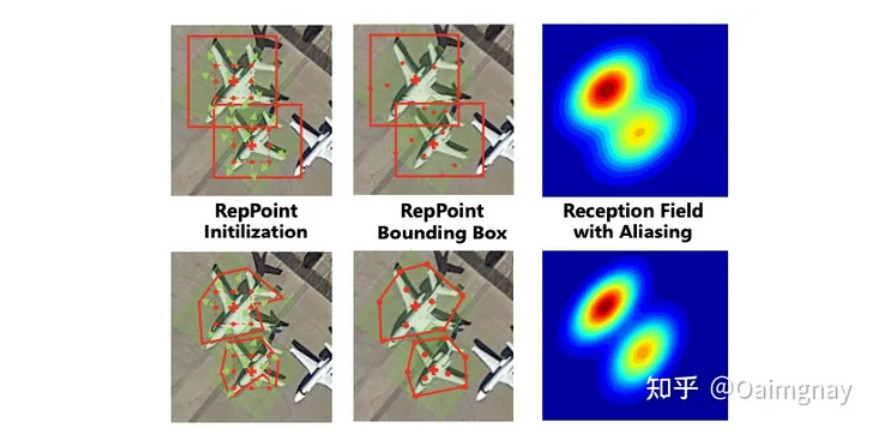
\includegraphics[width=400px]{./compare_cfa_with_other.JPG}
		\caption{Minh hoạ vấn đề. (Bên trên) Khi sử dụng cách biểu diễn dạng hộp, các đối tượng có hướng phân bố dày đặc gây ra hiện tượng đặc trưng răng cưa tại các vùng giao của trường tiếp nhận giữa các đối tượng. (Bên dưới) Với cách biểu diễn bao lồi, phương pháp CFA xử lý tốt các đặc trưng nằm trên lưới tích chập thông thường của các đối tượng có hướng phân bố không đều, giải quyết hiện tượng răng cưa đặc trưng hiệu quả}
		\label{fig_dhandang1}
	\end{center}
\end{figure} 


Để giải quyết các vấn đề trên, một phương pháp đã được đưa ra: phương pháp thích ứng bao lồi (convex-hull feature adaptation-CFA). CFA được thực hiện dựa trên phương pháp biểu diễn bao lồi, định nghĩa một tập các điểm đặc trưng, giới hạn phạm vi của đối tượng mục tiêu sử dụng chỉ số CIoU. CFA đạt được sự phân bổ đặc trưng tối ưu nhờ vào việc xây dựng tập bao lồi và phân chia linh hoạt các bao lồi thành các bao lồi âm và bao lồi dương. CFA cũng xem xét sự chồng chéo nhau giữa bao lồi dự đoán và bao lồi thực tế, phạt các bao lồi được dùng chung bởi nhiều đối tượng, giảm thiểu hiện tượng đặc trưng răng cưa (feature aliasing), đạt được sự thích ứng đặc trưng tối ưu. Nó cũng đạt được kết quả tốt nhất khi thử nghiệm trên tập dữ liệu DOTA và SKUR110KR.

Phương pháp CFA được chia làm 2 giai đoạn thực hiện:
\begin{itemize}
	\item Giai đoạn 1: tạo tập bao lồi và ước lượng sơ bộ bố cục của bao lồi.
	\item Giai đoạn 2: chỉnh sửa bao lồi sao cho phù hợp với các đối tượng phân bổ dày đặc.
\end{itemize}

\begin{figure}[ht!]
	\begin{center}
		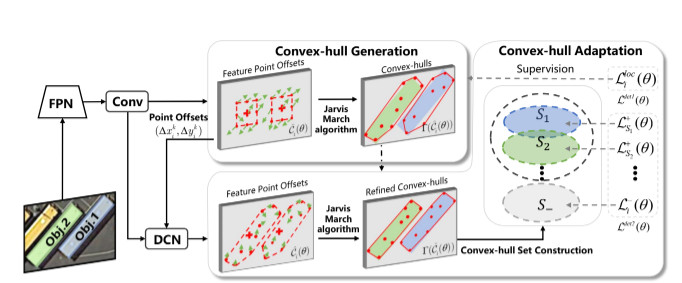
\includegraphics[width=450px]{./work_flow_cfa.JPG}
		\caption{Biểu đồ luồng quy trình thực hiện của bộ phát hiện CFA.}
		\label{work_flow_cfa}
	\end{center}
\end{figure} 

\section{Xây dựng tập bao lồi đầu tiên}
Việc biểu diễn bằng khung hình chữ nhật do bao lồi sinh ra làm giảm khả năng biểu diễn đối tượng. Vì thế phương pháp CFA đã đề xuất biểu diễn phạm vi của đối tượng bằng bao lồi. Mỗi bao lồi là một tập hợp các điểm thoả mãn công thức:

\begin{align} \label{convex_hull_definition}
		C_i=\left\{\left(x_i^k, y_i^k\right)\right\}_i^{k=1 \ldots K}
\end{align}
Trong đó: $C_i$ là bao lồi thứ i, $\left(x_i^k, y_i^k\right)$ là điểm nằm trên bao lồi thứ k, k là chỉ số của điểm đặc trưng, $K = 9$ tương ứng với 9 điểm được khởi tạo của bao lồi.

\begin{figure}[ht!]
	\begin{center}
		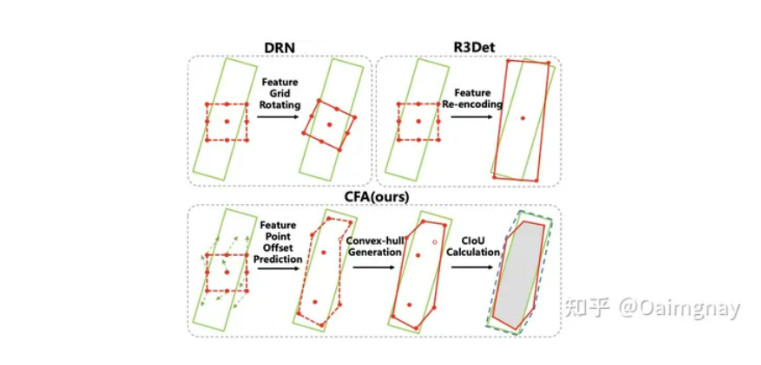
\includegraphics[width=445px]{./compare_convex-hull_with_rectangle.jpg}
		\caption{So sánh biểu diễn hộp có hướng (bên trên) so với biểu diễn bao lồi (ở dưới).}
	\end{center}
\end{figure} 


Việc huấn luyện có thể xem như là quá trình dự đoán độ lệch (offset), trong khi hệ số CIoU cần được tối đa hoá để đạt được so khớp tối ưu nhất. Đây là phương pháp sử dụng phép toán tích chập để dự đoán độ lệch:
$\left(\Delta x_i^k, \Delta y_i^k\right)$
với từng điểm đặc trưng, sau trả về một bản đồ độ bù cho các đặc trưng
$O \in R^{H \times W \times W}$ ($H, W, C$ lần lượt tương ứng với chiều dài, chiều rộng và số lượng kênh của bản đồ đặc trưng):
\begin{align} \label{convex_hull_learn_offset}
	\hat{\mathcal{C}}_i(\theta) \leftarrow\left\{\left(x_i^k+\Delta x_i^k(\theta), y_i^k+\Delta y_i^k(\theta)\right)\right\}_i^{k=1 \ldots K}
\end{align}

Trong đó: $\theta$ biểu thị là các tham số của mạng. Việc dự đoán offset sẽ thực hiện theo công thức trên.

\section{Tích chập biến dạng}
Tích chập biến dạng (Deformable convolution) là dạng tích chập mà vị trí thực hiện tích chập bị biến dạng, không giống tích chập truyền thống là dạng lưới $N\mathrm{x}N$. Ưu điểm của phương pháp này giúp trích xuất các đặc trưng mong muốn được chính xác hơn, lấy mẫu được ở những vị trí đa dạng hơn (Phép tích chập truyền thống chỉ có thể trích xuất các đặc trưng trên một khung hinh chữ nhật).(Hình \ref{so_sanh_tich_chap_thong_thuong_deformable})

\begin{figure}[ht!]
	\begin{center}
		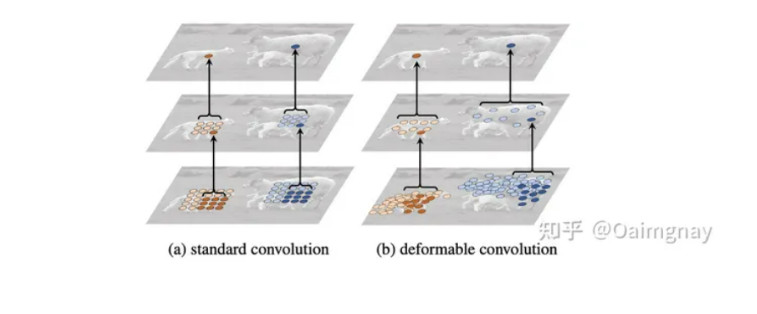
\includegraphics[width=445px]{./compare_normal_with_deformable_convolution.jpg}
		\caption{So sánh tích chập thông thường và tích chập biến dạng.}
		\label{so_sanh_tich_chap_thong_thuong_deformable}
	\end{center}
\end{figure} 

Phép tích chập biến dạng thực ra là thêm phần bù cho các điểm tích chập lấy mẫu. (Hình \ref{offset_deformable_convolution})

\begin{figure}[ht!]
	\begin{center}
		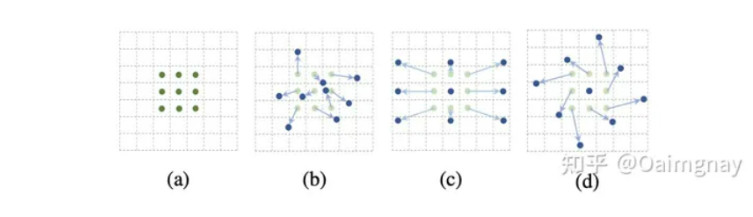
\includegraphics[width=445px]{./feature_offset_type.jpg}
		\caption{a) lấy mẫu tích chập với 9 điểm lấy mẫu. b) để có tích chập biến dạng, thêm độ dịch chuyển vào mỗi điểm lấy mẫu (mũi tên xanh). c) phép biến đổi tỷ lệ. d) phép quay
		}
		\label{offset_deformable_convolution}
	\end{center}
\end{figure} 

\begin{figure}[ht!]
	\begin{center}
		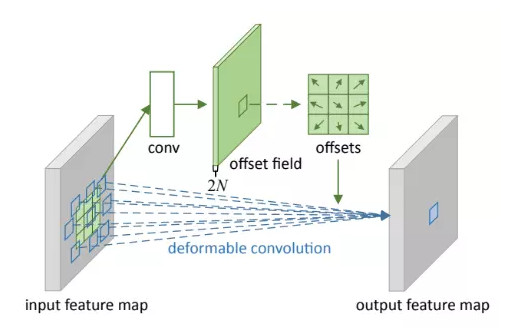
\includegraphics[width=400px]{./deformable_process.jpg}
		\caption{Quá trình thực hiện tích chập biến dạng.}
		\label{deformable_process}
	\end{center}
\end{figure} 


Cho đầu vào là một bản đồ đặc trưng, giả sử phép tích chập là 3x3. Để học được phần bù, định nghĩa một lớp tích chập 3x3 khác, chiều của đầu ra là kích thước của bản đồ đặc trưng ban đầu, số kênh = $2N$. (Hình \ref{deformable_process}) Tiếp theo thực hiện tích chập biến dạng, dựa trên độ bù của các phần đã được tính trước đó, sau đó thực hiện phép tích chập như thông thường.
\section{Thuật toán Jarvis March}
Sau khi học được phần bù, việc hoàn thành cập nhật các điểm đặc trưng của bao lồi được thực hiện bởi thuật toán Jarvis March, bao lồi nhỏ nhất phù hợp với điều kiện sẽ được tạo ra sau mỗi vòng lặp.

\begin{figure}[ht!]
	\begin{center}
		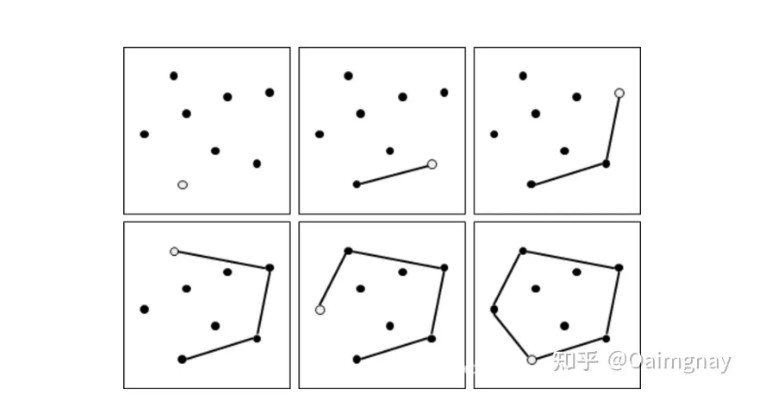
\includegraphics[width=435px]{./jarvis_march_steps.jpg}
		\caption{mô tả các bước thực hiện thuật toán Jarvis March}
		\label{fig_dhandang1}
	\end{center}
\end{figure} 
Tóm tắt các bước thực hiện thuật toán Jarvis March:

\begin{itemize}
	\item Bước 1: Chọn điểm xuất phát là v1 nằm trên đường biên. Tìm điểm v2 tiếp theo sao cho mọi điểm khác trong tập hợp nằm ở phía bên trái đoạn thằng nối v1 và v2.
	\item Bước 2: Tìm điểm v3 tiếp theo trong tập các điểm còn lại, sao cho v1, v2, v3 thỏa mãn góc ngược chiều kim đồng hồ (Counter Clock Wise - CCW). Điền này có nghĩa là v3 nằm ở bên trái đoạn thẳng nối v1 và v2. Nếu điều kiện này được đáp ứng, tức là v3 là 1 điểm nằm ở ngoại vi hơn.
	\item Bước 3: Nếu điều kiện bước trên thỏa mãn, ghi đè giá trị của v3 lên v2. Gán giá trị của v3 cho v2, tức v2 = v3. Quay lại bước 2 để tìm điểm ngoại vi tiếp theo.
	\item Bước 4: Lặp lại bước 3 cho đến khi tất cả các điểm đã được duyệt qua, tức là tìm thấy điểm ngoại vi tiếp theo được tìm thấy. Quá trình này tạo ra một chuỗi các điểm trên đường biên của bao lồi.
	\item Bước 5: Ghi đè giá trị của v2 lên v1. Sau khi tìm thấy điểm ngoại vi tiếp theo, gán giá trị của v2 lên v1, tức v1 = v2.
	\item  Bước 6: Lặp lại bước 2 cho đến khi điểm tiếp theo trả về chính là điểm xuất phát. Quá trình này sẽ tiếp tục cho đến khi ta quay trở lại điểm xuất phát ban đầu, hoàn thành toàn bộ quá trình tìm bao lồi.
\end{itemize}

\section{Đinh nghĩa công thức Convex Intersection over Union (CIoU)}
Dựa vào mỗi bao lồi dự đoán, có thể tính toán được hàm mất mát vị trí và phân lớp của một đối tượng. Công thức CIoU giữa bao lồi dự đoán thứ $i$:  $C_i(\theta)$ và hộp bao thật sự $\mathcal{B}_j$ của đối tượng thứ $j$ được tính như sau:

\begin{align} \label{CioU_fomular}
	\operatorname{CIoU}\left(\mathcal{C}_i(\theta), \mathcal{B}_j\right)=\frac{\left|\mathcal{C}_i(\theta) \cap \mathcal{B}_j\right|}{\left|\mathcal{C}_i(\theta) \cup \mathcal{B}_j\right|}-\frac{\left|\mathcal{R}_j \backslash\left(\mathcal{C}_i(\theta) \cup \mathcal{B}_j\right)\right|}{\left|\mathcal{R}_j\right|}
\end{align}
Trong đó: $\mathcal{R}_j$ là hợp của hai đa giác, tức là đa giác nhỏ nhất có thể bao quanh  $C_i(\theta)$ và $\mathcal{B}_j$.
\section{Hàm mất mát}
Theo công thức \ref{CioU_fomular}, hàm mất mát vị trí CIoU được định nghĩa là:
\begin{align} \label{cong_thuc_ham_loss_CIoU}
	\mathcal{L}_i^{l o c}(\theta)=1-\operatorname{CIoU}\left(\mathcal{C}_i(\theta), \mathcal{B}_j\right)
\end{align}
Cho $f_i^{k}(\theta)$ là đặc trưng của điểm thứ $k$, bao lồi đặc trưng $f_i(\theta)$ được tính bởi tổng có trọng số của tất cả các điểm đặc trưng trên bao lồi dự đoán $\mathcal{C}_i(\theta)$, tức là bằng công thức: $f_i(\theta) = \sum_{k}m w_i^k.f_i^k(\theta)$, trong đó, $w_i^k$ biểu thị các trọng số đặc trưng có thể học được từ tích chập biến dạng (DCN). Dựa vào bao lồi đặc trưng, điểm dự đoán $S_i(\theta)$ của bao lồi dự đoán $C_i(\theta)$ được tính bởi phép tích chập, hàm mất mát phân loại của bao lồi dự đoán $C_i(\theta)$ tương ứng với $B_j$ được định nghĩa là:
\begin{align} \label{loss_classification}
	\mathcal{L}_i^{c l s}(\theta)=\mathrm{FL}\left(S_i(\theta), Y_j\right)
\end{align}
ở đây $Y_j$ biểu thị là nhãn nhị phân thật sự (ground-truth) và FL() ở đây là hàm mất mát Focal (Focal loss). Kết quả có được là hàm mất mát dành cho bao lồi dương: 
\begin{align} \label{loss_function_positive_convex}
	\mathcal{L}_i^{+}(\theta)=\mathcal{L}_i^{c l s}\left(\mathcal{S}_i(\theta), Y_j\right)+\lambda \mathcal{L}_i^{l o c}\left(\mathcal{C}_i(\theta), \mathcal{B}_j\right)
\end{align}
Hàm mất mát \ref{loss_function_positive_convex} là tổng của hàm mất mát vị trí \ref{cong_thuc_ham_loss_CIoU} và hàm mất mát phân loại \ref{loss_classification}.
Hàm mất mát dành cho bao lồi âm là:

\begin{align} \label{loss_negative_convex}
	\mathcal{L}_i^{-}(\theta)=\mathcal{L}_i^{c l s}\left(\mathcal{S}_i(\theta), Y_j\right)
\end{align}
Ngoài ra, trong quá trình huấn luyện (Hình \ref{work_flow_cfa}), vì các bao lồi được ban đầu chỉ được sinh ra bằng cách tối ưu CIoU, một hàm loss cần được định nghĩa cho việc giám sát:
\begin{align} \label{loss_det_1}
	\mathcal{L}^{\operatorname{det} 1}(\theta)=\frac{1}{J} \sum_i \mathbb{I}_{\left(x_i, y_i\right)} \mathcal{L}_i^{l o c}(\theta)
\end{align}
Nhìn chung, trong giai đoạn đầu tiên của việc sinh bao lồi, hàm mất mát $L^{\operatorname{det} 1}$ bên trên là hàm cần được quan tâm. Trong giai đoạn 2, hai hàm mất mát phân lớp (\ref{loss_negative_convex} và \ref{loss_function_positive_convex}) sẽ được sử dụng để phân loại bao lồi
\section{Thích ứng bao lồi}
Phương pháp biểu diễn bằng bao lồi giúp định vị đối tượng ở bất kỳ hình dạng nào, tuy nhiên vẫn có một vấn đề, làm thế nào để định vị một cách chính xác các đối tượng dày đặc, đặc biệt là các đối tượng có đặc trưng răng cưa. Vì vậy bộ phát hiện CFA đã đề xuất một phương pháp thích ứng mới để tinh chỉnh các bao lồi sinh ra ở giai đoạn 1 để đạt được vị trí chính xác hơn và phân lớp hiệu quả hơn.
\subsection{Xây dựng tập các bao lồi}
Bộ phát hiện cho xây dựng một tập các bao lồi với mỗi đối tượng, để một đối tượng mục tiêu có thể khớp với nhiều bao lồi phù hợp để cùng nhau tối ưu các đặc trưng của các đối tượng dày đặc.

\begin{figure}[ht!]
	\begin{center}
		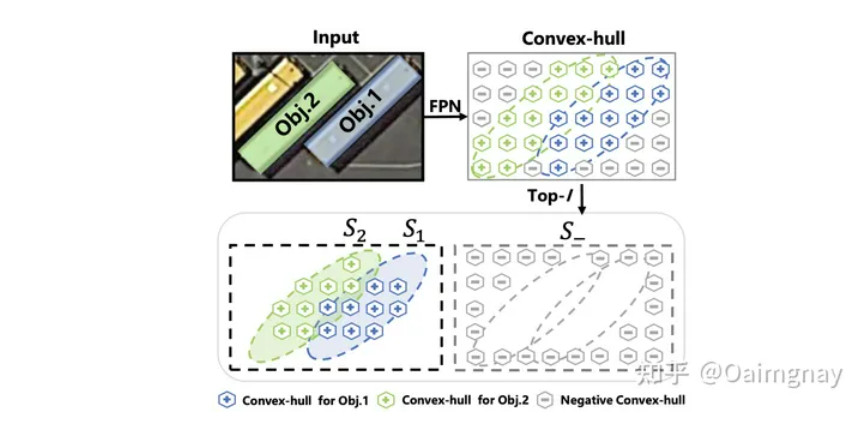
\includegraphics[width=445px]{./construction_convex_hull_set.jpg}
		\caption{xây dựng tập các bao lồi để biểu diễn các đối tượng, đặc biệt với những đối tượng phân bổ dày đặc}
		\label{fig_dhandang1}
	\end{center}
\end{figure} 
Với mỗi mục tiêu, ý tưởng xây dựng tập bao lồi tương ứng là: theo như hệ số CIoU giữa bao lồi dự đoán và bao lồi thực tế, chọn I bao lồi đứng đầu là ứng cử viên cho bao lồi dương để xây dựng tập các bao lồi. Ngoài ra cũng có thể xây dựng tập bao lồi sử dụng ngưỡng CIoU xác định bằng thực nghiệm. Các bao lồi còn lại không thuộc vào bất kỳ tập bao lồi nào sẽ được gộp lại thành tập bao lồi âm $S$.
\begin{align} \label{construct_convex_hull_set}
\mathcal{L}_{S_j}^{+}(\theta)=\frac{1}{\left|S_j\right|} \sum_{i \in S_j} \omega_i \mathcal{L}_i^{+}(\theta)
\end{align}
Khi nhiều đối tượng tập hợp lại cùng nhau, không phải tất cả các bao lồi nằm trong tập bao lồi đều phù hợp với đối tượng, và các bao lồi có đặc trưng răng cưa sẽ phải được phân loại thành tập các bao lồi âm. Cùng thời điểm đó, các bao lồi được chia sẻ bởi nhiều đối tượng phải phải có độ tin cậy thấp hơn.
\subsection{Chiến lược phân đoạn tập các bao lồi}
Để giải quyết vấn đề đặc trưng răng cưa ở các đối tượng dày đặc, bộ phát hiện CFA đề xuất chiến lược phân đoạn tập các bao lồi để đánh giá động các mẫu bao lồi âm và mẫu dương, chuyển đổi trọng số $\omega_i$ thành $f\left(L_i^{+}(\theta)\right)$. Sau khi thay thế, được công thức sau:
\begin{align} \label{loss_positive_convert}
	\mathcal{L}_{s_j}^{+}(\theta)=\frac{1}{\left|S_j\right|} \sum_{i \in S_j} f\left(\mathcal{L}_i^{+}(\theta)\right) \mathcal{L}_i^{+}(\theta)
\end{align}
Trong đó: $f$ là hàm lỗi đơn điệu giảm phân phối Gaussian: $f\left(x\right) = 1.0 - \frac{2}{\sqrt{\pi}}\int_0^xe^{-t^2}$, có nghĩa là giá trị mất càng nhỏ, độ tin cậy càng cao.

\begin{figure}[ht!]
	\begin{center}
		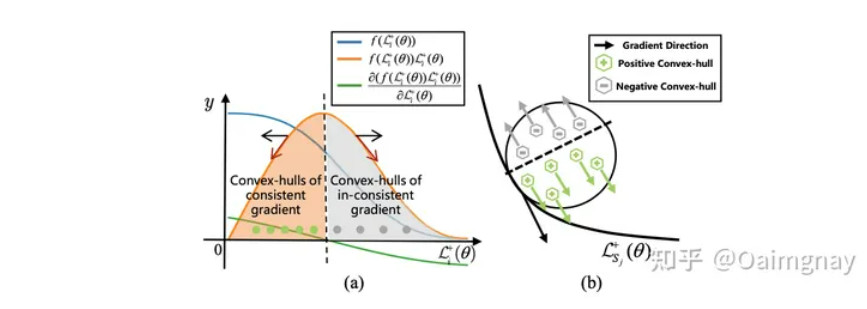
\includegraphics[width=445px]{./gaussian_gradient.jpg}
		\caption{Phân chia tập bao lồi theo hướng dẫn của nguyên tắc nhất quán độ dốc.}
		\label{gradient_consistentcy_illustration}
	\end{center}
\end{figure} 
Nguyên tắc phân chia tập bao lồi là nguyên tắc nhất quá độ dốc. Bằng cách lấy đạo hàm của công thức công thức \ref{loss_positive_convert}, ta có được:
\begin{align} \label{gradient_of_loss}
	 \frac{\partial \mathcal{L}_{s_j}^{+}(\theta)}{\partial \theta}=\frac{1}{\left|S_j\right|} \sum_{i \in S_j} \frac{\partial\left(f\left(\mathcal{L}_i^{+}(\theta)\right) \mathcal{L}_i^{+}(\theta)\right)}{\partial \mathcal{L}_i^{+}(\theta)} \frac{\partial \mathcal{L}_i^{+}(\theta)}{\partial \theta}
\end{align}
Tiêu chí để thực hiện phân đoạn tập các bao lồi là: đạo hàm của mỗi một bao lồi dương $\frac{\partial L_i^{+}(\theta)}{\partial \theta}$ yêu cầu đạo hàm của toàn bộ tập bao lồi $\frac{\partial L_{S_j}^{+}(\theta)}{\partial \theta}$ là nhất quán. Điều này có nghĩa là: bao lồi nào có độ dốc không nhất quán được xem là bao lồi âm, tức là những bao lồi này sẽ dẫn đến hiện tượng răng cưa đặc trưng. Xem xét công thức \ref{gradient_of_loss}, nếu $\frac{\partial\left(f\left(L_i^{+}(\theta)\right) L_i^{+}(\theta)\right)}{\partial L_i^{+}(\theta)}$ mang giá trị dương, thì bao lồi $C_i$ được xếp là bao lồi dương, hoặc ngược lại bao lồi sẽ là âm. Xem xét hình \ref{gradient_consistentcy_illustration}, khi sắp xếp các giá trị mất mát  $\frac{\partial L_i^{+}(\theta)}{\partial \theta}$ theo thứ tự tăng dần, $f\left(\partial L_i^{+}(\theta)\right) L_i^{+}(\theta)$ (đường màu cam) là một hàm lồi hướng lên với một cực trị duy nhất, trong khi đường  $\frac{\partial\left(f\left(L_i^{+}(\theta)\right) L_i^{+}(\theta)\right)}{\partial L_i^{+}(\theta)}$ (màu xanh lục) chia các bao lồi thành tập các bao lồi dương $S_j$ và tập bao lồi âm $S\_$.

Cùng thời điểm đó, để xử lý đặc trưng răng cưa, tác giả cũng giới thiệu hệ số chống đặc trưng răng cưa:
\begin{align}\label{FAA_fomular}
	p_i = \gamma\dot{\frac{\mathrm{CIoU}(\mathcal{C}_i, \mathcal{B}_j)}{\sum_{m=1}^{M}\mathrm{CIoU}\left(\mathcal{C}_i, \mathcal{B}_j\right)}}
\end{align}
Hệ số này thể hiện mức độ mà một đối tượng thuộc về một đối tượng duy nhất, khi nó chồng lên M đối tượng khác. $\gamma$ là hệ số chống đặc trưng răng cưa.
Hàm mất mát được cập nhật thành: 

\begin{align}\label{loss_update}
	\mathcal{L}_{s_j}^{+}(\theta)=\frac{1}{\left|S_j\right|} \sum_{i \in S_j} p_i f\left(\mathcal{L}_i^{+}(\theta)\right) \mathcal{L}_i^{+}(\theta)
\end{align}
Giai đoạn 2 của quá trình tối ưu được điều khiển bởi hàm mất mát trên tập bao lồi, hàm này được xác định bằng cách kết hợp hàm mất mát phân loại và hàm mất mát vị trí:
\begin{align} \label{loss_det_2}
	\begin{aligned}
		\mathcal{L}^{\operatorname{det} 2}(\theta)= & \frac{1}{J} \sum_{j=1}^J \frac{1}{\left|S_j\right|} \sum_{i \in S_j} p_i f\left(\mathcal{L}_i^{+}(\theta)\right) \mathcal{L}_i^{+}(\theta) \\
		& +\frac{1}{\left|S_{-}\right|} \sum_{i \in S_{-}} \mathcal{L}_i^{-}(\theta)
	\end{aligned}
\end{align}

Hàm mất mát này xem xét sự tương ứng về đặc trưng của nhiều đối tượng, tiến hành phạt các bao lồi được chia sẻ bởi nhiều đối tượng, và giảm thiểu đặc trưng răng cưa để đạt được thích ứng đặc trưng tối ưu. Cuối cùng hàm mất mát của toàn bộ bộ phát hiện CFA là: 
\begin{align} \label{final_loss_CFA}
	L^{\operatorname{det} 1}(\theta)+L^{\operatorname{det} 2}(\theta)
\end{align}

\chapter{Thuật toán tính bao lồi xấp xỉ}
\textit{Giới thiệu chung về thuật toán, cách dùng, có bao nhiêu loại thuật toán}
\section{Outer convex approximation}
Cho:
\begin{align} \label{ct2.1} 
	X:=\left\{x_1, x_2, \ldots, x_n\right\} \subset \mathbb{R}^2
\end{align}
Giả sử không mất tính tổng quát rằng
\begin{align} \label{ct2.2} 
	x_1, x_2, \ldots, x_n  \text{ không cùng nằm trên cùng một đường thẳng.}
\end{align}
Ta viết tất cả các vector thành dạng vector hàng, những vector này sẽ có chuyển vị của chúng được ký hiệu bởi chỉ số trên $T$, và sử dụng chỉ số trên để chỉ định các thành phần của chúng, ví dụ: $x = \left(x^1, x^2\right)\in\mathbb{R}^2$. Cho $x, x'\in\mathbb{R}^2$, chứng tỏ:
\begin{equation}\label{ct2.3}
	\begin{aligned}
		& {\left[x, x^{\prime}\right]:=\left\{(1-\lambda) x+\lambda x^{\prime} \mid \lambda \in[0,1]\right\}} \\
		& \left(x, x^{\prime}\right):=\left\{(1-\lambda) x+\lambda x^{\prime} \mid \lambda \in(0,1)\right\}
	\end{aligned}
\end{equation}

Cho $X$ thỏa mãn (\ref{ct2.1}) - (\ref{ct2.2}) và $\delta \geq 0$, trong phần này em muốn tìm một bao lồi xấp xỉ của $X$, nghĩa là:
\begin{align}\label{ct2.4}
	\text{Một đa giác lồi }\mathcal{P}^{outer} \text{thỏa mãn bao lồi }X\subset\mathcal{P}^{outer}
\end{align}
sao cho
\begin{align}\label{ct2.5}
	dist_H\left(conv\ X, \mathcal{P}^{outer}\right) \leq \delta
\end{align}
$P^{outer}$ đươc xác định bởi:
\begin{align}\label{ct2.6}
	P^{outer} := \{x\in\mathbb{R}^2 | dx^T \leq \beta_d\ \text{ với tất cả d} \in D\}
\end{align}
Trong đó $D \subset \mathbb{R^2}$ biểu thị tập các hướng tối đa và $\beta_d \in \mathbb{R}$ biểu thị ngưỡng tương ứng với hướng $d \in D$. Với D cho trước, $\mathcal{P}^{outer}$ là bao lồi xấp xỉ phù hợp nhất chứa $X$ nếu:
\begin{equation}\label{ct2.7}
	\beta_d:=\max _{x \in X} d x^T \text{với tất cả d }\in D
\end{equation}
Cho P là tập các đỉnh của $\mathcal{P}^{outer}$.
Ta bắt đầu quá trình xác định bao lồi xấp xỉ ngoài với hình chữ nhật nhỏ nhất có chứa $X$, tập $X$ này có chứa cạnh song song với trục tọa độ. Theo công thức (\ref{ct2.5}) - (\ref{ct2.6}), hình chữ nhật $\mathcal{P}^{outer}$ được xác định bởi:
\begin{align}\label{ct2.8}
	D:=\{(1, 0), (0, 1), (-1, 0), (0, -1)\}
\end{align}
và:
\begin{equation}\label{ct2.9}
	\begin{aligned}
		& \beta_{(1,0)}:=\max \left\{x^1 \mid\left(x^1, x^2\right) \in X\right\}, \\
		& \beta_{(0,1)}:=\max \left\{x^2 \mid\left(x^1, x^2\right) \in X\right\}, \\
		& \beta_{(-1,0)}:=\max \left\{-x^1 \mid\left(x^1, x^2\right) \in X\right\}, \\
		& \beta_{(0,-1)}:=\max \left\{-x^2 \mid\left(x^1, x^2\right) \in X\right\} .
	\end{aligned}
\end{equation}
Theo công thức (\ref{ct2.2}) ta có:

\begin{center}
	$\beta_{(-1, 0)} \textless \beta_{(1, 0)}$ \text{ và } $\beta_{(0, -1)} \textless \beta_{(0, 1)}$
\end{center}
Vì vậy, ${P}^{outer}$ là một hình chữ nhật phù hợp với 4 đỉnh phân biệt, có tập đỉnh là:
\begin{align}\label{ct2.10}
	P := \{r_1, r_2, r_3, r_4\}
\end{align}
Trong đó:
\begin{equation}\label{ct2.11}
	\begin{aligned}
		& r_1:=\left(\beta_{(1,0)}, \beta_{(0,1)}\right), \\
		& r_2:=\left(\beta_{(-1,0)}, \beta_{(0,1)}\right), \\
		& r_3:=\left(\beta_{(-1,0)}, \beta_{(0,-1)}\right), \\
		& r_4:=\left(\beta_{(1,0)}, \beta_{(0,-1)}\right) .
	\end{aligned}
\end{equation}
Trong các bước xấp xỉ tiếp theo, việc xây dựng đa giác ${P}^{outer}$ lần lượt được cải thiện như sau:

$\text{Với 1 đỉnh }p \in P, \text{cho } p^{-} \in P \text{ và } p^{+} \in P \text{ lần lượt là}$
\begin{align} \label{ct2.12}
\text {điểm liền trước ngược chiều kim đồng hồ và điểm liền sau của} p \in P.
\end{align}. 


Ta có công thức sau:
\begin{equation}\label{ct2.13}
	\begin{array}{lcl}
		d_{p}^T &:=& \|p^+ - p^-\|^{-1}\, R \, (p^+ - p^-)^T, \\
		\beta_{d_{p}} &:=& \max\{d_{p}\, x^T \mid x \in X\},
	\end{array}
\end{equation}
Trong đó:
\begin{equation}\label{ct2.14}
	R := \begin{pmatrix}
		0 & 1 \\
		-1 & 0
	\end{pmatrix}
\end{equation}
là ma trận xoay chiều theo hướng kim đồng hồ với góc xoay $\pi/2$. Vì $R$ là ma trận xoay, ta có:
\begin{equation}\label{ct2.15}
	\|d_{p}\| = \|p^+ - p^-\|^{-1}\, \|(p^+ - p^-) R^T\| = \|p^+ - p^-\|^{-1}\, \|p^+ - p^-\| = 1.
\end{equation}
Sẽ có hai trường hợp xảy ra khi ta thêm các ràng buộc tuyến tính sau đây vào định nghĩa của ${P}^{outer}$ trong công thức (\ref{ct2.6}):
\begin{equation}\label{ct2.16}
	d_p\, x^T \leq \beta_{d_p}.
\end{equation}

Đầu tiên, nếu:
\begin{equation}\label{ct2.17}
	\beta_{d_p} = d_p\, p^+
\end{equation}
thì công thức (\ref{ct2.15}) không tạo thêm đỉnh mới nhưng sẽ thêm 2 cạnh mới  $[p^-, p^+]$ của ${\cal P}^{\rm outer}$. Cho  $d_{[p^-, p]}$ và $d_{[p, p^+]}$ biểu thị 2 hướng cực đại từ D, định nghĩa hai cạnh $[p^-, p]$ và $[ p, p^+]$ của ${\cal P}^{\rm outer}$. Sau đó $d_{[p^-, p]}$ and $d_{[p, p^+]}$ sẽ trở nên vô dụng. Vì vậy, trong khi thêm $d_p$ vào tập $D$ cần phải loại bỏ $d_{[p^-, p]}$ và $d_{[p, p^+]}$ và $p$ trong $P$, nghĩa là:
\begin{equation}\label{ct2.18}
	\begin{array}{lcl}
		D &:=& (D \cup \{d_{p}\})\setminus \{d_{[p^-,p]}, d_{[p,p^+]}\}, \\
		P &:=& P \setminus \{p\}.
	\end{array}
\end{equation}
Thứ hai, nếu
\begin{equation}\label{ct2.19}
	\beta_{d_p} > d_p\, p^+
\end{equation}
và:
\begin{equation}\label{ct2.20}
	d_{p}\, p^T - \beta_{d_{p}} > \delta
\end{equation}
thì ràng buộc mới (\ref{ct2.16}) tạo ra hai đỉnh mới của ${\cal P}^{\rm outer}$ có tên $\hat p^-$ và $\hat p^+$ sẽ được tính như sau:
\begin{equation}\label{ct2.21}
	\begin{array}{lcl}
		\lambda_p &:=& (\beta_{d_p} - d_p\, p^{-T})/(d_p\, p^T - d_p\, p^{-T}) \in (0, 1), \\
		\hat p^- &:=& (1 - \lambda_p)\, p^{-T} + \lambda_p\, p^T, \\
		\hat p^+ &:=& (1 - \lambda_p)\, p^{+T} + \lambda_p\, p^T.
	\end{array}
\end{equation}

Do đó, ta sẽ cộng $d_p$ vào $D$ và thay $p \in P$ bằng $\hat p^-$ và $\hat p^+$.
\begin{equation}\label{ct2.22}
	\begin{array}{lcl}
		D &:=& D \cup \{d_{p}\}, \\
		P &:=&(P \setminus \{p\}) \cup \{\hat p^-, \hat p^+\}.
	\end{array}
\end{equation}

Quy trình xấp xỉ được mô tả trong thuật toán sau, trong đó $P_{\rm doubt}$ biểu thị tập hợp các đỉnh vẫn cần được kiểm tra.

\begin{algorithm}\label{alg01}  \rm 
		\floatname{algorithm}{Thuật toán}
		\caption{}  \label{al-blduoi0}
	\emph{Input:} Tập hữu hạn $X \subset \R^2$ và tham số xấp x $\delta \geq 0$. \\
	\emph{Output:} Đa giác xấp xỉ lồi ${\cal P}^{\rm outer}$ được xác định ở công thức (\ref{ct2.6}) bởi $D$ và $\beta_d$ cho $d \in D$ và tập đỉnh $P$.
	\begin{enumerate}
		\item\label{stepIalg01} 
		Xác định $D$, $\beta_d$ với $d \in D$, và $P$ theo (\ref{ct2.8})--(\ref{ct2.11}).
		
		\item\label{stepIIalg01} Đặt $P_{\rm doubt} := P$.
		
		\item\label{stepIIIalg01} 
		 Chọn ngẫu nhiên một đỉnh $p \in P_{\rm doubt}$  và tham chiếu lên $d_p$, $\beta_{d_p}$ theo (\ref{ct2.12})--(\ref{ct2.14}). \\
		Nếu (\ref{ct2.17}) là đúng thì thay đổi $D$, $P$ như (\ref{ct2.18}), và cập nhập
		\begin{equation}\label{ct2.23}
			P_{\rm doubt} := P_{\rm doubt} \setminus \{p, p^-, p^+\},
		\end{equation}
		Và đi tới bước \ref{stepIValg01}.\\
		Nếu % (\ref{betagreater}) and 
		(\ref{ct2.20}) là đúng thì thay đổi $D$, $P$ như (\ref{ct2.22}), cập nhật
		\begin{equation}\label{ct2.24}
			P_{\rm doubt} := (P_{\rm doubt} \setminus \{p\}) \cup \{\hat p^-, \hat p^+\},
		\end{equation}
		Và đi tới bước \ref{stepIValg01}.\\
		Nếu không thì, 
		\begin{equation}\label{ct2.25}
			P_{\rm doubt} := P_{\rm doubt} \setminus \{p\}.
		\end{equation}
		
		\item\label{stepIValg01} 
		Nếu $P_{\rm doubt}$ chưa rỗng thì quay lại bước \ref{stepIIIalg01}.
		
		\item
		 Trả về tập hợp các hướng cực đại $D$ và $\beta_d$ với $d \in D$, tập đỉnh $P$ của ${\cal P}^{\rm outer}$, và kết thúc thuật toán.
	\end{enumerate}
\end{algorithm}

Với (\ref{ct2.6}) - (\ref{ct2.7}), mỗi cạnh $\left[p, p^{+}\right]$ của $\mathcal{P}$ chứa ít nhất một điểm của tập $X$. Do đó, (\ref{ct2.11}) suy ra:
$$
\beta_{d_p} \geq d_p p^{-}=d_p p^{+} .
$$
Do đó, nếu (\ref{ct2.17}) sai thì (\ref{ct2.19}) hiển nhiên đúng. Điều này giải thích tại sao (\ref{ct2.19}) không cần kiểm tra cùng với (\ref{ct2.20}) ở bước \ref{stepIIIalg01}.
Thuật toán 1 có thể nhanh chóng tạo ra một đa giác lồi xấp xỉ $\mathcal{P}^{\text {outer }}$ với $d_p p^T-\beta_{d_p} \leq \delta$ với tất cả $p \in P$.
Tính chất này là cần thiết nhưng không đủ cho (\ref{ct2.5}). Để đảm bảo (\ref{ct2.5}), trong thuật toán tiếp theo chúng ta cũng kiểm tra xem nếu 
\begin{equation}\label{ct2.26}
	\begin{array}{lcl}
	 \|p-x\|>\delta \text { với mọi } x \in X_p, \quad \text { trong đó } \\
	 X_p:=\left\{x \in X \mid d_p x^T=\beta_{d_p}\right\} .
	\end{array}
\end{equation}

\begin{algorithm}\label{alg02}  \rm 
	\floatname{algorithm}{Thuật toán}
	\caption{}  \label{al-blduoi1}
	\emph{Input:}  Tập hữu hạn $X \subset \R^2$ và tham số xấp xỉ $\delta \geq 0$. \\
	\emph{Output:} Đa giác xấp xỉ lồi  ${\cal P}^{\rm outer}$  được xác định ở công thức (\ref{ct2.6}) bởi $D$ và $\beta_d$ cho $d \in D$ và tập đỉnh $P$.
	\begin{enumerate}
		\item\label{stepIalg02} 
		Xác định $D$, $\beta_d$ với $d \in D$, và $P$ theo (\ref{ct2.8})--(\ref{ct2.11}).
		
		\item\label{stepIIalg02} Đặt $P_{\rm doubt} := P$.
		
		\item\label{stepIIIalg02} 
		Chọn ngẫu nhiên một đỉnh $p \in P_{\rm doubt}$ và tham chiếu lên $d_p$, $\beta_{d_p}$ theo (\ref{ct2.12})--(\ref{ct2.14}). \\
		Nếu (\ref{ct2.17}) là đúng thì thay đổi $D$, $P$ như (\ref{ct2.18}), và cập nhật
		\begin{equation}\label{ct2.27}
			P_{\rm doubt} := P_{\rm doubt} \setminus \{p, p^-, p^+\},
		\end{equation}
		Và đi tới bước \ref{stepIValg02}.\\
		Nếu (\ref{ct2.20}) à đúng thì thay đổi $D$, $P$ như (\ref{ct2.22}), và cập nhật
		\begin{equation}\label{ct2.28}
			P_{\rm doubt} := (P_{\rm doubt} \setminus \{p\}) \cup \{\hat p^-, \hat p^+\},
		\end{equation}
		Và đi tới bước \ref{stepIValg02}.\\
		Nếu (\ref{ct2.26}) là đúng thì thay đổi $D$, $P$ như (\ref{ct2.22}), và cập nhật $P_{\rm doubt}$ theo (\ref{ct2.28}), và đi tới bước \ref{stepIValg02}.\\
		Nếu không thì cập nhập, 
		\begin{equation}\label{ct2.29}
			P_{\rm doubt} := P_{\rm doubt} \setminus \{p\}.
		\end{equation}
		
		\item\label{stepIValg02} 
		Nếu $P_{\rm doubt}$ chưa rỗng thì quay lại bước \ref{stepIIIalg02}.
		
		\item
		Trả về tập hợp các hướng cực đại $D$ và $\beta_d$ với $d \in D$, tập đỉnh $P$ của ${\cal P}^{\rm outer}$, kết thúc thuật toán.
	\end{enumerate}
\end{algorithm}

\begin{figure}[ht!]
	\begin{center}
		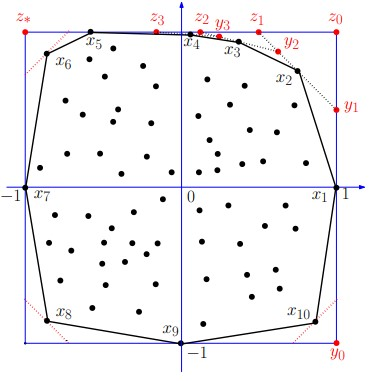
\includegraphics[width=300px]{./convex X.jpg}
		\caption{$X = \{x_1, x_2, \dots, x_n\}$ with $\ conv X = \ conv\{x_1, x_2, \dots, x_m\}$ and $m = 10$.}
		\label{fig_dhandang2_1}
	\end{center}
\end{figure}

\medskip
Để minh họa tác dụng của thuật toán \ref{al-blduoi0}--\ref{al-blduoi1}, chúng ta hãy coi $X$ là một tập hợp $n$ các điểm ngẫu nhiên trong đa giác khung $16$ cạnh ${\cal P}^\diamond$ được thể hiện 
trong hình \ref{fig_dhandang2_2}.\\

\begin{figure}[ht!]
	\begin{center}
		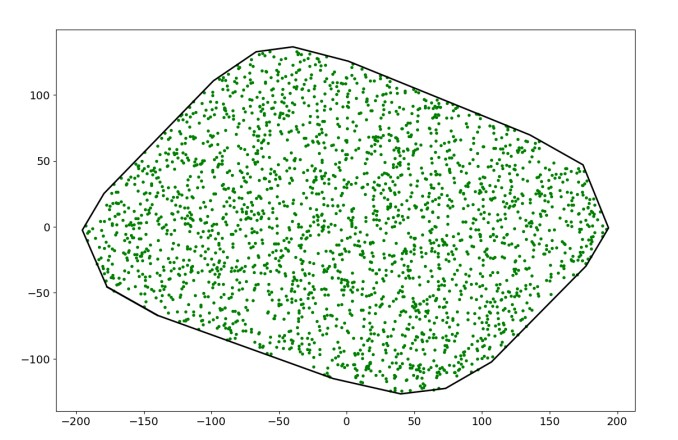
\includegraphics[width=300px]{./Frame pylogon.jpg}
		\caption{$16$-sided frame polygon ${\cal P}^\diamond$ of $n$ random points.}
		\label{fig_dhandang2_2}
	\end{center}
\end{figure}
\medskip
Bảng \ref{table01} cho thấy một số kết quả thử nghiệm, trong đó
\begin{itemize}
	\item $\#_{\rm Edges@ Alg.\, 1}$ là số cạnh của đa giác xấp xỉ lồi bao ngoài ${\cal P}^{\rm outer}$ được trả về bởi thuật toán \ref{al-blduoi0},
	\item $\#_{\rm Edges@ Alg.\, 2}$ là số cạnh của đa giác xấp xỉ lồi bao ngoài ${\cal P}^{\rm outer}$ được tả về bởi thuật toán \ref{al-blduoi1},
	\item $\#_{\rm Step\, III @ Alg.\, 1}$  là số lần thực hiện của bước 3 trong thuật toán \ref{al-blduoi0}
	\item $\#_{\rm Step\, III @ Alg.\, 2}$ là số lần thực hiện của bước 3 trong thuật toán \ref{al-blduoi1}.
\end{itemize}
\begin{table}[ht]
	\begin{center}\renewcommand{\arraystretch}{1.2}\small
		\setlength\tabcolsep{0.05cm}
		\begin{tabular}{|c|c||c|c|c|c|c|c|c|c|c|c|c|c|c|}
			%\hline
			\hline
			\multicolumn {2}{|c||}{\footnotesize $\#X=n$}  & ???& ???& ???& ???& ???& ???& ???& ???& ???& ???& ??? \\ 
			\hline		
			\hline
			{ $\delta = ???$}
			
			& $\#_{\rm Edges@ Alg.\, 1}$  &   ???& ???& ???& ???& ???& ???& ???& ???& ???& ???& ??? \\
			
			& $\#_{\rm Edges@ Alg.\, 2}$  &   ???& ???& ???& ???& ???& ???& ???& ???& ???& ???& ??? \\
			
			& $\#_{\rm Step\, III @ Alg.\, 1}$  &   ???& ???& ???& ???& ???& ???& ???& ???& ???& ???& ??? \\
			
			& $\#_{\rm Step\, III @ Alg.\, 2}$& ???& ???& ???& ???& ???& ???& ???& ???& ???& ???& ???   \\
			\hline
			{ $\delta = ???$}
			
			& $\#_{\rm Edges@ Alg.\, 1}$  &   ???& ???& ???& ???& ???& ???& ???& ???& ???& ???& ??? \\
			
			& $\#_{\rm Edges@ Alg.\, 2}$  &   ???& ???& ???& ???& ???& ???& ???& ???& ???& ???& ??? \\
			
			& $\#_{\rm Step\, III @ Alg.\, 1}$  &   ???& ???& ???& ???& ???& ???& ???& ???& ???& ???& ??? \\
			
			& $\#_{\rm Step\, III @ Alg.\, 2}$& ???& ???& ???& ???& ???& ???& ???& ???& ???& ???& ???   \\
			\hline
			{ $\delta = ???$}
			
			& $\#_{\rm Edges@ Alg.\, 1}$  &   ???& ???& ???& ???& ???& ???& ???& ???& ???& ???& ??? \\
			
			& $\#_{\rm Edges@ Alg.\, 2}$  &   ???& ???& ???& ???& ???& ???& ???& ???& ???& ???& ??? \\
			
			& $\#_{\rm Step\, III @ Alg.\, 1}$  &   ???& ???& ???& ???& ???& ???& ???& ???& ???& ???& ??? \\
			
			& $\#_{\rm Step\, III @ Alg.\, 2}$& ???& ???& ???& ???& ???& ???& ???& ???& ???& ???& ???   \\
			\hline
			{ $\delta = 0$}
			
			& $\#_{\rm Edges@ Alg.\, 1}$  &   ???& ???& ???& ???& ???& ???& ???& ???& ???& ???& ??? \\
			
			& $\#_{\rm Edges@ Alg.\, 2}$  &   ???& ???& ???& ???& ???& ???& ???& ???& ???& ???& ??? \\
			
			& $\#_{\rm Step\, III @ Alg.\, 1}$  &   ???& ???& ???& ???& ???& ???& ???& ???& ???& ???& ??? \\
			
			& $\#_{\rm Step\, III @ Alg.\, 2}$& ???& ???& ???& ???& ???& ???& ???& ???& ???& ???& ???   \\
			\hline
		\end{tabular}
		\caption{Số cạnh của đa giác lồi xấp xỉ ${\cal P}^{\rm outer}$ được trả về bởi thuật toán \ref{al-blduoi0}--\ref{al-blduoi1} và số lần thực hiện của bước \ref{stepIIIalg01} khi $X$ gồm $n$ điểm ngẫu nhiên trong khung $16$ cạnh đa giác ${\cal P}^\diamond$ thể hiện trong hình \ref{fig_dhandang2_2}.}
		\label{table01}
	\end{center}
\end{table} 	



	\bigskip\noindent
	{\bf LƯU Ý: (Liên quan đến bảng \ref{table01}):} 
	 $n$ điểm ngẫu nhiên trong bảng \ref{table01} phải được tạo ra trong đa giác ${\cal P}^\diamond$ với khung 16 cạnh như trong hình \ref{fig_dhandang2_2}.
	
	\bigskip


Nếu số điểm $n$ của $X$ rất lớn thì việc tính toán $\beta_{d_{p}}$ xác định trong (\ref{ct2.13}) sẽ tốn kém, có thể giảm đang kể như sau. Lấy bốn điểm  $q_1$, $q_2$, $q_3$, và $q_4$ của $X$ nằm trên bốn cạnh của hình chữ nhập ban đầu ${\cal P}^{\rm outer}$, tức là.
\begin{equation}\label{ct2.30}
	q_1, q_2, q_3, q_4 \in X
\end{equation}
and
\begin{equation}\label{ct2.31}
	\begin{array}{lcl}
		(1, 0)\, q_1^T &=& \beta_{(1, 0)}, \\
		(0, 1)\, q_2^T &=& \beta_{(0, 1)}, \\
		(-1, 0)\, q_3^T &=& \beta_{(-1, 0)}, \\
		(0, -1)\, q_4^T &=& \beta_{(0, -1)}.
	\end{array}
\end{equation}
Với $j \in \{1, 2, 3, 4\}$ và $q_5 := q_1$, nếu $q_j \not= q_{j+1}$ thì xác định
\begin{equation}\label{ct2.32}
	X_j := \{x \in X \mid \bar d_{[q_j, q_{j+1}]}\, (x - q_j)^T \geq 0\}, 
\end{equation}
Trong đó
\begin{equation}\label{ct2.33}
	\bar d_{[q_j, q_{j+1}]}^{\, T} := \|q_{j+1} - q_j\|^{-1} R\, (q_{j+1} - q_j)^T.
\end{equation}
Trong thuật toán tiếp thep, $X$ trong (\ref{ct2.12}) và (\ref{ct2.26}) được thay thế bằng $X_j$, tức là
\begin{equation}\label{ct2.34}
	\begin{array}{lcl}
		d_{p}^T &:=& \|p^+ - p^-\|^{-1} R \, (p^+ - p^-)^T, \\
		\beta_{d_{p}} &:=& \max\{d_{p}\, x^T \mid x \in X_j\}, 
	\end{array}
\end{equation}
và
\begin{equation}\label{ct2.35}
	\begin{array}{lcl}
		&& \|p - x\| > \delta \ \mbox{ với mọi } x \in X_p, \ \mbox{ trong đó} \\
		&& X_p := \{x \in X_j \mid d_{p}\, x^T = \beta_{d_{p}}\},
	\end{array}
\end{equation}
Với $j \in \{1, 2, 3, 4\}$.

\begin{algorithm}\label{alg03}  \rm 
	\floatname{algorithm}{Thuật toán}
	\caption{}  \label{al-blduoi2}
	\emph{Input:}  Tập hữu hạn $X \subset \R^2$ và tham số xấp xỉ  $\delta \geq 0$. \\
	\emph{Output:} Đa giác xấp xỉ lồi ${\cal P}^{\rm outer}$ được xác định bởi công thức (\ref{ct2.6}) bởi $D$ và $\beta_d$ cho $d \in D$ và tập đỉnh $P$.
	\begin{enumerate}
		\item\label{stepIalg03} 
		Xác định $D$, $\beta_d$ với $d \in D$, $r_j$ theo $j \in \{1, 2, 3, 4\}$, và $P$ bởi (\ref{ct2.8})--(\ref{ct2.11}). \\
		Cho $j := 1$ và $q_5 := q_1$. 
		
		\item\label{stepIIalg03} 
		Nếu $q_j = q_{j+1}$ thì đi tới bước \ref{stepValg03}.\\
		Nếu không thì, xác định $X_j$ bởi (\ref{ct2.30})--(\ref{ct2.32}) và tập $P_{\rm doubt} := \{r_j\}$.
		
		\item\label{stepIIIalg03} 
		Chọn ngẫu nhiên một đỉnh $p \in P_{\rm doubt}$ và được xác định ở công thức $d_p$, $\beta_{d_p}$ bởi (\ref{ct2.12}) và (\ref{ct2.34}). \\
	Nếu
		\begin{equation*}%\label{betaequal+}
			\beta_{d_p} = d_p\, p^-
		\end{equation*}
		thì thay đổi $D$ và $P$ như (\ref{ct2.18}), và cập nhật
		\begin{equation*}\label{ct2.36}
			P_{\rm doubt} := P_{\rm doubt} \setminus \{p, p^-, p^+\}
		\end{equation*}
		và đi tới bước \ref{stepIValg03}.\\
		Nếu 
		\begin{equation*}%\label{greaterdelta+}
			d_{p}\, p^T - \beta_{d_{p}} > \delta
		\end{equation*}
		thì thay đổi $D$ và $P$ như (\ref{ct2.22}), và cập nhât 
		\begin{equation}\label{newPdoubt4+}
			P_{\rm doubt} := (P_{\rm doubt} \setminus \{p\}) \cup \{\hat p^-, \hat p^+\}
		\end{equation}
		và đi tới bước \ref{stepIValg03}.\\
		Nếu (\ref{ct2.35}) đúng thì thay đổi $D$, $P$ như (\ref{ct2.22}), và cập nhật $P_{\rm doubt}$ theo (\ref{ct2.36}), và đi tới bước \ref{stepIValg03}.\\
		Nếu không thì,
		\begin{equation*}%\label{newPdoubt6+}
			P_{\rm doubt} := P_{\rm doubt} \setminus \{p\}.
		\end{equation*}
		
		\item\label{stepIValg03} 
		Nếu $P_{\rm doubt}$ là khác rỗng thì chuyển sang bước \ref{stepIIIalg03}.
		
		\item\label{stepValg03} 
		Nếu $j < 4$ then $j := j+1$ và đi đến bước \ref{stepIIalg03}.
		
		\item\label{stepVIalg03} 
		 Trả về tập hợp các hướng cực đại $D$ và $\beta_d$ với $d \in D$, và tập đỉnh $P$ của ${\cal P}^{\rm outer}$, và kết thúc thuật toán.
	\end{enumerate}
\end{algorithm}
\medskip
Bảng \ref{table02} và hình\ref{Figure03} cho thấy một số kết quả thử nghiệm về thời gian chay của thuật toán \ref{al-blduoi1}--\ref{al-blduoi2} khi $X$ bao gồm $n$ điểm ngẫu nhiên trong đa giác khung $16$ cạnh của ${\cal P}^\diamond$ được hiển thị trong hình \ref{Figure02}, trong đó
\begin{itemize}
	\item $T_{\rm Alg.\, 2}$ là thời gian chạy trung bình của thuật toán \ref{al-blduoi1},
	\item $T_{\rm Alg.\, 3}$ là thời gian chạy trung bình của thuật toán \ref{al-blduoi2}.
\end{itemize}

\begin{table}[ht]
	\begin{center}\renewcommand{\arraystretch}{1.2}\small
		\setlength\tabcolsep{0.05cm}
		\begin{tabular}{|c|c||c|c|c|c|c|c|c|c|c|c|c|c|c|}
			%\hline
			\hline
			\multicolumn {2}{|c||}{\footnotesize $\#X=n$}  & ???& ???& ???& ???& ???& ???& ???& ???& ???& ???& ??? \\ 
			\hline		
			\hline
			{ $\delta = ???$}
			
			& $T_{\rm Alg.\, 2}$  &   ???& ???& ???& ???& ???& ???& ???& ???& ???& ???& ??? \\
			
			& $T_{\rm Alg.\, 3}$  &   ???& ???& ???& ???& ???& ???& ???& ???& ???& ???& ??? \\
			
			& $T_{\rm Alg.\, 2}/n$  &   ???& ???& ???& ???& ???& ???& ???& ???& ???& ???& ??? \\
			
			& $T_{\rm Alg.\, 3}/n$& ???& ???& ???& ???& ???& ???& ???& ???& ???& ???& ???   \\
			\hline
			{ $\delta = ???$}
			
			& $T_{\rm Alg.\, 2}$  &   ???& ???& ???& ???& ???& ???& ???& ???& ???& ???& ??? \\
			
			& $T_{\rm Alg.\, 3}$  &   ???& ???& ???& ???& ???& ???& ???& ???& ???& ???& ??? \\
			
			& $T_{\rm Alg.\, 2}/n$  &   ???& ???& ???& ???& ???& ???& ???& ???& ???& ???& ??? \\
			
			& $T_{\rm Alg.\, 3}/n$& ???& ???& ???& ???& ???& ???& ???& ???& ???& ???& ???   \\
			\hline
			{ $\delta = ???$}
			
			& $T_{\rm Alg.\, 2}$  &   ???& ???& ???& ???& ???& ???& ???& ???& ???& ???& ??? \\
			
			& $T_{\rm Alg.\, 3}$  &   ???& ???& ???& ???& ???& ???& ???& ???& ???& ???& ??? \\
			
			& $T_{\rm Alg.\, 2}/n$  &   ???& ???& ???& ???& ???& ???& ???& ???& ???& ???& ??? \\
			
			& $T_{\rm Alg.\, 3}/n$& ???& ???& ???& ???& ???& ???& ???& ???& ???& ???& ???   \\
			\hline
			{ $\delta = 0$}
			
			& $T_{\rm Alg.\, 2}$  &   ???& ???& ???& ???& ???& ???& ???& ???& ???& ???& ??? \\
			
			& $T_{\rm Alg.\, 3}$  &   ???& ???& ???& ???& ???& ???& ???& ???& ???& ???& ??? \\
			
			& $T_{\rm Alg.\, 2}/n$  &   ???& ???& ???& ???& ???& ???& ???& ???& ???& ???& ??? \\
			
			& $T_{\rm Alg.\, 3}/n$& ???& ???& ???& ???& ???& ???& ???& ???& ???& ???& ???   \\
			\hline
		\end{tabular}
		\caption{Thời gian chạy trung bình $T_{\rm Alg.\, 2}$ và $T_{\rm Alg.\, 3}$ của thuật toán \ref{al-blduoi1} và thuật toán \ref{al-blduoi2}
			khi $X$ gồm $n$ điểm ngẫu nhiên trong đa giác có khung $16$ cạnh của ${\cal P}^\diamond$ hiển thị như hình \ref{fig_dhandang2_2}.}
		\label{table02}
	\end{center}
\end{table} 
\begin{figure}[ht]
	\centering
	???
	%\includegraphics[width=8cm]{./Figures/???}
	\caption{Tỷ lệ thời gian chạy của thuật toán \ref{al-blduoi1}--\ref{al-blduoi2} và số điểm $n$ của $X$.}
	\label{Figure03}
\end{figure}


	\bigskip\noindent
	{\bf LƯU Ý (liên quan đến bảng \ref{table02} và hình \ref{Figure03}):} 
	
	- $n$ điểm ngẫu nhiên được trình bày ở bảng \ref{table02} phải được tạo theo phương trình xoay trong đa giác có khung $16$ cạnh của  ${\cal P}^\diamond$ được hiển thị tỏng hình \ref{fig_dhandang2_2}.
	
	- Chỉ có hai tỷ lệ $T_{\rm Alg.\, 2}/n$ và $T_{\rm Alg.\, 3}/n$ được trình bày trong hình \ref{Figure03}.
	
	\bigskip

======================================================





\section{Inner convex approximation}\label{InnerConvexApproximation}

Cho $X$ thỏa mãn (\ref{ct2.1})--(\ref{ct2.2}) và $\delta \geq 0$, ở đây ta sẽ tìm một xấp xỉ lồi trong ${\cal P}^{\rm inner}$  của $X$, tức là:
\begin{equation}\label{ct2.37}
	{\cal P}^{\rm inner} := \ conv X', \ \mbox{ với} X' \subset X,
\end{equation}
Thật vậy
\begin{equation}\label{ct2.38}
	\ dist_{\rm H}(\ conv X, {\cal P}^{\rm inner}) \leq \delta.
\end{equation}

Ta mô tả ${\cal P}^{\rm inner}$ bởi tập $E$ của các cạnh có hướng của nó $[p, p^+]$, trong đó $p^+$  là cạnh kế tiếp ngược chiều kim đồng hồ của $p$, tức là:
\begin{equation}\label{ct2.39}
	E := \{[p, p^+] \mid p, p^+ \in X', \mbox{ $[p, p^+]$ là một cạnh của ${\cal P}^{\rm inner}$}\}.
\end{equation}


Ta bắt đầu quá trình xấp xỉ lồi trong với tứ giác $\bar q_1 \bar q_2 \bar q_3 \bar q_4$, tức là:
\begin{equation}\label{ct2.40}
	\begin{array}{lcl}
		X' &:=& \{\bar q_1, \bar q_2, \bar q_3, \bar q_4\}, \\
		E &:=& \{[\bar q_1, \bar q_2], \, [\bar q_2, \bar q_3], \, [\bar q_3, \bar q_4], \, [\bar q_4, \bar q_1]\},
	\end{array}
\end{equation}
Trong đó $\bar q_1$, $\bar q_2$, $\bar q_3$, và $\bar q_4$ là duy nhất và được xác định bởi:
\begin{equation}\label{ct2.41}
	\begin{array}{lcl}
		x^1_{\rm min} &:=& \min \{x^1 \mid (x^1, x^2) \in X\}, \\
		x^1_{\rm max} &:=& \max \{x^1 \mid (x^1, x^2) \in X\}, \\
		x^2_{\rm min} &:=& \min \{x^2 \mid (x^1, x^2) \in X\}, \\
		x^2_{\rm max} &:=& \max \{x^2 \mid (x^1, x^2) \in X\}
	\end{array}
\end{equation}
Và
\begin{equation}\label{ct2.42}
	\begin{array}{lcl}
		X^1_{\rm min} &:=& \{(x^1, x^2) \in X \mid x^1 = x^1_{\rm min}\}, \\
		X^1_{\rm max} &:=& \{(x^1, x^2) \in X \mid x^1 = x^1_{\rm max}\}, \\
		X^2_{\rm min} &:=& \{(x^1, x^2) \in X \mid x^2 = x^2_{\rm min}\}, \\
		X^2_{\rm max} &:=& \{(x^1, x^2) \in X \mid x^2 = x^2_{\rm max}\}
	\end{array}
\end{equation}
Và
\begin{equation}\label{ct2.43}
	\begin{array}{lcl}
		&& \bar q_1 = (\bar q_1^1, \bar q_1^2) \in X^1_{\rm max} \mbox{ thỏa mãn } \bar q_1^2 = \max\{x^2 \mid (x^1, x^2) \in X^1_{\rm max}\}, \\
		&& \bar q_2 = (\bar q_2^1, \bar q_2^2) \in X^2_{\rm max} \mbox{  thỏa mãn} \bar q_2^1 = \min\{x^1 \mid (x^1, x^2) \in X^2_{\rm max}\}, \\
		&& \bar q_3 = (\bar q_3^1, \bar q_3^2) \in X^1_{\rm min} \mbox{  thỏa mãn } \bar q_3^2 = \min\{x^2 \mid (x^1, x^2) \in X^1_{\rm min}\}, \\
		&& \bar q_4 = (\bar q_4^1, \bar q_4^2) \in X^2_{\rm min} \mbox{  thỏa mãn } \bar q_4^1 = \max\{x^1 \mid (x^1, x^2) \in X^2_{\rm min}\}.
	\end{array}
\end{equation}
Lưu ý rằng hai trong số bốn điểm $\bar q_1$, $\bar q_2$, $\bar q_3$, và $\bar q_4$ có thể trùng nhau, nhưng (\ref{ct2.2}) ngụ ý rằng ít nhất ba trong số chúng khác nhau.

Trong các bước xấp xỉ sau đây, đa giác ${\cal P}^{\rm inner}$ được xây dựng và cải thiện 
như sau.
Với bất kỳ $[p, p^+] \in E$ ($p \not= p^+$), ta các định:
\begin{equation}\label{ct2.44}
	\begin{array}{lcl}
		\bar d_{[p, p^+]}^{\, T} &:=& \|p^+ - p\|^{-1} R \, (p^+ - p)^T, \\
		X_{[p, p^+]} &:=& \{x \in X \mid \bar d_{[p, p^+]}\, x^T > \bar d_{[p, p^+]}\, p^T \},
	\end{array}
\end{equation}
Với
\begin{equation*}%\label{rotationmatrix}
	R := \begin{pmatrix}
		0 & 1 \\
		-1 & 0
	\end{pmatrix}.
\end{equation*}

Nếu $X_{[p, p^+]} \not= \emptyset$ thì xác định
\begin{equation}\label{ct2.45}
	\begin{array}{lcl}
		\beta_{[p, p^+]} &:=& \max \{\bar d_{[p, p^+]}\, x^T \mid x \in X_{[p, p^+]}\}, \\
		B_{[p, p^+]} &:=& \{x \in X_{[p, p^+]} \mid \bar d_{[p, p^+]}\, x^T = \beta_{[p, p^+]}\}.
	\end{array}
\end{equation}
Nếu
\begin{equation}\label{dct2.46}
	\beta_{[p, p^+]} - \bar d_{[p, p^+]}\, p^T \leq \delta
\end{equation}
Thì ta không cần phải mở rộng ${\cal P}^{\rm inner }$ theo hướng $\bar d_{[p, p^+]}$.

Ngược lại, nếu
\begin{equation}\label{ct2.47}
	\beta_{[p, p^+]} - \bar d_{[p, p^+]}\, p^T > \delta
\end{equation}
thì lấy  
\begin{equation}\label{ct2.48}
	\hat p \in B_{[p, p^+]} \hbox{ thỏa mãn } \|\hat p - p\| = \max\{\|x - p\| \mid x \in B_{[p, p^+]}\},
\end{equation}
Và cập nhập $X'$ và $B$ bởi
\begin{equation}\label{ct2.49}
	\begin{array}{lcl}
		X' &:=& X' \cup \{\hat p\}, \\
		E &:=& E \cup \{[p, \hat p], \, [\hat p, p^+]\},
	\end{array}
\end{equation}
Và xác định
\begin{equation}\label{ct2.50}
	\begin{array}{lcl}
		X_{[p, \hat p]} &:=& \{x \in X_{[p, p^+]} \mid \bar d_{[p, \hat p]}\, x^T > \bar d_{[p, \hat p]}\, p^T \}, \\
		X_{[\hat p, p^+]} &:=& \{x \in X_{[p, p^+]} \mid \bar d_{[\hat p, p^+]}\, x^T > \bar d_{[\hat p, p^T]}\, {\hat p}^T \}.
	\end{array}
\end{equation}
Lưu ý rằng ta chỉ xem xét $x \in X_{[p, p^+]}$ trong định nghĩa này của $X_{[p, \hat p]}$ vaf $X_{[\hat p, p^+]}$, nhưng tất cả $x \in X$ trong định nghĩa (\ref{ct2.44}) của $X_{[p, p^+]}$.

Quy trình xấp xỉ được trình bày trong thuật toán sau, trong đó  $E_{\rm doubt}$ biểu thị tập hợp các cạnh vẫn cần được kiểm tra.

\begin{algorithm}\label{alg04}  \rm 
	\floatname{algorithm}{Thuật toán}
	\caption{}  \label{al-blduoi4}
	\emph{Input:} Tập hữu hạn $X \subset \R^2$ và tham số xấp xỉ $\delta \geq 0$. \\
	\emph{Output:} Đa giác xấp xỉ lồi trong ${\cal P}^{\rm inner}$ được mô tả bởi $X'$ và $E$.
	\begin{enumerate}
		\item\label{stepIalg04} 
		Xác định $X'$ và $E$ theo (\ref{ct2.40})--(\ref{ct2.43}).\\
		Với mọi $[p, p^+] \in E$ xác định $d_{[p, p^+]}$ và $X_{[p, p^+]}$ theo (\ref{ct2.44}).\\
		Cho $E_{\rm doubt} := E$.
		
		\item\label{stepIIalg04} 
		 Chọn tùy ý $[p, p^+] \in E_{\rm doubt}$. \\
		Nếu $X_{[p, p^+]} = \emptyset$ thì đặt
		$E_{\rm doubt} := E_{\rm doubt} \setminus \{[p, p^+]\}$
		và đi tới bước \ref{stepIIIalg04}.\\
		Định nghĩa $\beta_{[p, p^+]}$ và $B_{[p, p^+]}$ theo (\ref{ct2.45}). \\
		Nếu (\ref{dct2.46}) đúng thì đặt
		$E_{\rm doubt} := E_{\rm doubt} \setminus \{[p, p^+]\}$
		Và đi tới bước \ref{stepIIIalg04}.\\
		Trường hợp còn lại, lấy $\hat p$ định nghĩa theo (\ref{ct2.48}),
		và cập nhật $X'$ và $E$ theo (\ref{ct2.49}), và xác định $X_{[p, \hat p]}$ và $X_{[\hat p, p^+]}$ theo (\ref{ct2.50}),	và đặt
		\begin{equation*}%\label{newBdoubt3}
			E_{\rm doubt} := (E_{\rm doubt} \setminus \{[p, p^+])\}) \cup \{[p, \hat p], \, [\hat p, p^+]\}.
		\end{equation*}
		
		\item\label{stepIIIalg04} 
		Nếu $E_{\rm doubt}$ chưa rỗng thì quay lại bước \ref{stepIIalg04}.
		
		\item
		Trả về $X'$, $E$, và kết thúc thuật toán
	\end{enumerate}
\end{algorithm}


\medskip
Bảng \ref{table03}  cho thấy một số kết quả thử nghiệm, trong đó
\begin{itemize}
	\item $\#_{\rm Edges@ Alg.\, 4}$  là số cạnh trung bình của đa giác xấp xỉ lồi bao ngoài ${\cal P}^{\rm inner}$ được trả về bởi thuật toán \ref{al-blduoi4},
	\item $\#_{\rm Step\, II @ Alg.\, 4}$ à số lần thực hiện trung bình của bước \ref{stepIIalg04} của thuật toán \ref{al-blduoi4}.
\end{itemize}

\begin{table}[ht]
	\begin{center}\renewcommand{\arraystretch}{1.2}\small
		\setlength\tabcolsep{0.05cm}
		\begin{tabular}{|c|c||c|c|c|c|c|c|c|c|c|c|c|c|c|}
			%\hline
			\hline
			\multicolumn {2}{|c||}{\footnotesize $\#X=n$}  & ???& ???& ???& ???& ???& ???& ???& ???& ???& ???& ??? \\ 
			\hline		
			\hline
			{ $\delta = ???$}
			
			& $\#_{\rm Edges@ Alg.\, 4}$  &   ???& ???& ???& ???& ???& ???& ???& ???& ???& ???& ??? \\
			
			& $\#_{\rm Step\, II @ Alg.\, 4}$& ???& ???& ???& ???& ???& ???& ???& ???& ???& ???& ???   \\
			\hline
			{ $\delta = ???$}
			
			& $\#_{\rm Edges@ Alg.\, 4}$  &   ???& ???& ???& ???& ???& ???& ???& ???& ???& ???& ??? \\
			
			& $\#_{\rm Step\, II @ Alg.\, 4}$& ???& ???& ???& ???& ???& ???& ???& ???& ???& ???& ???   \\
			\hline
			{ $\delta = ???$}
			
			& $\#_{\rm Edges@ Alg.\, 4}$  &   ???& ???& ???& ???& ???& ???& ???& ???& ???& ???& ??? \\
			
			& $\#_{\rm Step\, II @ Alg.\, 4}$& ???& ???& ???& ???& ???& ???& ???& ???& ???& ???& ???   \\
			\hline
			{ $\delta = 0$}
			
			& $\#_{\rm Edges@ Alg.\, 4}$  &   ???& ???& ???& ???& ???& ???& ???& ???& ???& ???& ??? \\
			
			& $\#_{\rm Step\, II @ Alg.\, 4}$& ???& ???& ???& ???& ???& ???& ???& ???& ???& ???& ???   \\
			\hline
		\end{tabular}
		\caption{Số cạnh trung bình của đa giác lồi xấp xỉ lồi trong ${\cal P}^{\rm inner}$ Trả về bởi thuật toán \ref{al-blduoi4} và số lần thực hiện trung bình của bước \ref{stepIIalg04} khi $X$ gồm $n$ điểm ngẫu nhiên trong đa giác có khung $16$ cạnh ${\cal P}^\diamond$ và được hiển thị trong hình \ref{fig_dhandang2_2}.}
		\label{table03}
	\end{center}
\end{table} 	

	\bigskip\noindent
	{\bf LƯU Ý (Liên quan đến bảng \ref{table03}):}  $n$ điểm ngẫu nhiên được trình bày trong bảng \ref{table03} phải được tạo ra trong đa giác có khung $16$ cạnh ${\cal P}^\diamond$ và hiển thị trong hình \ref{fig_dhandang2_2}.
	
	\bigskip

\medskip
Bảng \ref{table04} và hình \ref{Figure04}  thể hiện một số kết quả thực nghiệm về thời gian chạy của thuật toán  \ref{alg04} khi $X$ gồm $n$ điểm ngẫu nhiên được trình bày trong bảng \ref{table03} phải được tạo ra trong đa giác có khung $16$ cạnh ${\cal P}^\diamond$ hiển thị trong hình \ref{fig_dhandang2_2}, trong đó

$T_{\rm Alg.\, 4}$ là thời gian chạy trung bình của thuật toán \ref{al-blduoi4}.

\begin{table}[ht]
	\begin{center}\renewcommand{\arraystretch}{1.2}\small
		\setlength\tabcolsep{0.05cm}
		\begin{tabular}{|c|c||c|c|c|c|c|c|c|c|c|c|c|c|c|}
			%\hline
			\hline
			\multicolumn {2}{|c||}{\footnotesize $\#X=n$}  & ???& ???& ???& ???& ???& ???& ???& ???& ???& ???& ??? \\ 
			\hline		
			\hline
			{ $\delta = ???$}
			
			& $T_{\rm Alg.\, 4}$  &   ???& ???& ???& ???& ???& ???& ???& ???& ???& ???& ??? \\
			
			& $T_{\rm Alg.\, 4}/n$& ???& ???& ???& ???& ???& ???& ???& ???& ???& ???& ???   \\
			\hline
			{ $\delta = ???$}
			
			& $T_{\rm Alg.\, 4}$  &   ???& ???& ???& ???& ???& ???& ???& ???& ???& ???& ??? \\
			
			& $T_{\rm Alg.\, 4}/n$& ???& ???& ???& ???& ???& ???& ???& ???& ???& ???& ???   \\
			\hline
			{ $\delta = ???$}
			
			& $T_{\rm Alg.\, 4}$  &   ???& ???& ???& ???& ???& ???& ???& ???& ???& ???& ??? \\
			
			& $T_{\rm Alg.\, 4}/n$& ???& ???& ???& ???& ???& ???& ???& ???& ???& ???& ???   \\
			\hline
			{ $\delta = ???$}
			
			& $T_{\rm Alg.\, 4}$  &   ???& ???& ???& ???& ???& ???& ???& ???& ???& ???& ??? \\
			
			& $T_{\rm Alg.\, 4}/n$& ???& ???& ???& ???& ???& ???& ???& ???& ???& ???& ???   \\
			\hline
		\end{tabular}
		\caption{Thời gian chạy trung bình $T_{\rm Alg.\, 4}$  thuật toán \ref{al-blduoi4} khi $X$ gồm $n$ điểm ngẫu nhiên được trình bày trong bảng \ref{table03} phải được tạo ra trong đa giác có khung $16$ cạnh  ${\cal P}^\diamond$ hiển thị trong hình \ref{fig_dhandang2_2}.}
		\label{table04}
	\end{center}
\end{table} 	

\begin{figure}[ht]
	\centering
	???
	%\includegraphics[width=8cm]{./Figures/???}
	\caption{Tỷ lệ thời gian chạy của thuật toán \ref{al-blduoi4} với số điểm $n$ của $X$.}
	\label{Figure04}
\end{figure}




\chapter{Ứng dụng .................}

Chương này trình bày định nghĩa và các tính chất của thặng dư bậc hai: cách tính thặng dư bằng định nghĩa, cách tính thặng dư thông qua ký hiệu Legendre, cách tính thông qua luật thuận nghịch bậc hai. Sau đó ứng dụng thặng dư bậc hai và luật thuận nghịch bậc hai để tính toán và giải một số bài toán chứng minh, tìm căn nguyên thủy, kiểm tra tính nguyên tố.  

\section{Thặng dư bậc hai và ứng dụng}
Thặng dư bậc hai đóng vai trò rất quan trọng trong lý thuyết số. Chẳng hạn, thuật toán phân tích số nguyên ra thừa số nguyên tố. Ngoài ra thặng dư bậc hai cũng ứng dụng lớn trong mật mã cũng như trong các giao thức mã hóa.... Ở đây ta xét ứng dụng liên quan đến giải phương trình đồng dư bậc hai trong lý thuyết và thực hành.
 
\subsection{Phương trình đồng dư bậc hai..........}
Xét phương trình đồng dư bậc hai theo modulo nguyên tố (theo tài liệu \cite{K2007}).
\begin{align}\label{pt7.1}
Ax^2 + Bx + C \equiv 0 \pmod{p},
\end{align}
trong đó $p$ nguyên tố lẻ và $A, B, C \in \mathbb{Z}$ với $p\nmid A$. (Nếu $p\mid A$ thì quay về phương trình tuyến tính). Vì $p$ nguyên tố lẻ và $p\nmid A$, nên $p\nmid 4A$. Ta nhân hai vế của phương trình với $4A$ ta được
\begin{equation}\label{pt7.2}
4A(Ax^2+Bx+C)\equiv 0\pmod p.
\end{equation}
Nhưng ta có 
\begin{align*}
4A(Ax^2+Bx+C)&=4A^2x^2+4ABx+4AC\\
&=(2Ax+B)^2-(B^2-4AC).
\end{align*}
Do đó đồng dư thức (\ref{pt7.2}) được viết lại thành
\begin{align*}
(2Ax+B)^2\equiv (B^2-4AC)\pmod p
\end{align*}
nó có dạng 
\begin{align}\label{pt7.3}
y^2\equiv a\pmod p
\end{align}
 trong đó $y=2Ax+B$ và $a=B^2-4AC$.\par 
Nếu phương trình $y^2\equiv a\pmod p$ có nghiệm, thì ta suy ra phương trình $2Ax+B=y$ có nghiệm $x$ modulo $p$ (vì $(2A,p)=1$). Do đó phương trình (\ref{pt7.1}) có nghiệm nếu và chỉ nếu phương trình (\ref{pt7.3}) có nghiệm.\par

Ví dụ sau sẽ minh họa điều này.

	{\fontsize{12pt}{12pt}\selectfont \baselineskip 0.65cm
	\renewcommand{\baselinestretch}{1.0}	
	\begin{algorithm}[ht!]
		
		\floatname{algorithm}{Thuật toán}
		\caption{\textsc{Thuật toán tìm bao lồi dưới} $\hbox{conv}_L(P)$}  \label{al-blduoi}
		\textbf{Đầu vào: }Cho $P=\{p_i=(x_i,y_i,z_i)\in \mathbb{R}^3,\ i=1,\dots,n\}, n\ge 3$.\\
		\textbf{Đầu ra:} Tập ${\cal Q}$ tất cả các mặt dưới của $\hbox{conv}_L(P)$.
		
		\begin{algorithmic}[1]
			
			
			\State Tìm cạnh đầu tiên $e_0$ của $\hbox{conv}_L(P)$. 
			\State Xét hàng đợi ${\cal Q}:=\emptyset$ và tập ${\cal E}_L(P):=\emptyset$.
			
			\State Gọi {\bf LFRes}($e, P$) để nhận được một mặt dưới $F_e$ qua $e_0$. Đẩy các cạnh của $F_e$  trừ $e_0$ vào trong ${\cal E}_L(P)$. Đẩy $F_e$ vào trong tập ${\cal Q}$.
			
			\State  {\bf while} $({\cal Q}\ne\emptyset)$ {\bf do}
			
			\State 
			\quad \quad Lấy $F_e$ từ phía trên của  ${\cal Q}$.
			
			\State 	\quad \quad \quad \quad $T:=$ tập các cạnh $F_e$.
			
			\State 	\quad \quad \quad \quad {\bf for each} $e \in T\cap  {\cal E}_L(P)$ {\bf do}
			
			\State 
			\quad \quad\quad \quad\quad \quad Gọi {\bf LFRes}($e, P$) để nhận được mặt $F'_e$ có chung cạnh $e$ với $F_e$. \hspace*{2.5cm}Đưa vào ${\cal E}_L(P)$ tất cả các cạnh $e' \ne e_0$ của $F'_e$ chưa xuất hiện trong \hspace*{2.5cm} ${\cal E}_L(P)$ và xoá các cạnh đã xuất hiện trong ${\cal E}_L(P)$. Đẩy $F'_e$ vào ${\cal Q}$.
		
			
		\end{algorithmic}
	\end{algorithm}
}

	\chapter{Một số kết quả tính toán }
Trong nội dung này chúng tôi thử nghiệm số cho thuật toán trong \cite{An-Giang} và thuật toán vừa được trình bày ở mục trước để so sánh tốc độ của chúng. Các thuật toán này được thực thi bởi chương trình C và chạy trên PC Core i5 1.6 GHz 3M với 4 GB RAM.  

Dưới đây Bảng \ref{tab:51} minh họa thời gian chạy (đơn vị tính bằng giây) của thuật toán tính bao lồi dưới được giới thiệu bởi P. T. An và D. T. Giang trong \cite{An-Giang} và Thuật toán \ref{al-matduoi} sử dụng kỹ thuật hạn chế của chúng tôi. Cột cuối cùng liệt kê tỉ lệ tăng tốc của thuật toán của chúng tôi so với thuật toán trong \cite{An-Giang}. Dữ liệu đầu vào của các thuật toán là các tập điểm được tạo trên bề mặt một paraboloid (tất cả các điểm đều là đỉnh của bao lồi và bao lồi dưới) có dạng $P = \{p_i = (x_i, y_i, z_i): x_i, y_i, z_i \in \mathbb{R}, z_i = x_i^2 + y_i^2, i = 1, \ldots, n\} \subset \mathbb{R}^3,$ trong đó tập $\{(x_i, y_i), x_i, y_i \in R, i = 1, \ldots , n \}$ được chọn ngẫu nhiên từ phân bố đều trong hình vuông cỡ 200 $\times$ 200. 

{\fontsize{12pt}{12pt}\selectfont \baselineskip 0.65cm
	\renewcommand{\baselinestretch}{1}
	\begin{table}[ht!]
		\begin{center}
			\caption{Thời gian chạy tính bao lồi dưới (đơn vị: giây).}
			\label{tab:51}
			\begin{tabular}{cccc}
				\hline
				{Đầu vào} &{Thuật toán trong} \cite{An-Giang} & {Thuật toán} \ref{al-blduoi}& Tỉ số thăng tốc\\
				\hline
				1.000 & 0,136& 0,061&2,23\\ 
				2.000 & 0,454& 0,248 &1,83\\  
				5.000 & 2,684& 1,500 &1,79\\  
				7.000 & 7,014& 3,129 &2,24\\ 
				11.000  & 14,321& 8,484 &1,69\\ 
				17.000  & 41,307& 24,666 &1,67\\ 
				20.000 & 63,197& 37,332 &1,69\\  
				22.000 & 70,866& 40,235 & 1,76\\ 
				30.000 & 153,240& 96,738 &1,58\\ 
				35.000& 200,496& 125,490& 1,60\\ \hline	
			\end{tabular}	
		\end{center}
	\end{table}	
}







\chapter*{{Kết luận}}
\addcontentsline{toc}{chapter}{\vspace*{-8pt} Kết luận}

 Trong quá trình thực tập, em đã có cơ hội làm quen một môi trường làm việc mới. Em đã tính lũy những kinh nghiệm về kiến thức trong công việc cũng như các kinh nghiệm về kỹ năng mềm.
 
 Em được rèn luyện kĩ năng giải quyết công việc theo từng giai đoạn, cố gắng hoàn thành công việc trong thời gian cho phép, mạnh dạn trao đổi và chia sẻ kiến thức. Đồng thời cũng bồi dưỡng thêm rất nhiều kiến thức ngoài các kiến thức đã học trên trường.
 




\begin{thebibliography}{30}
\addcontentsline{toc}{chapter}{\vspace*{-8pt} Tài liệu tham khảo}
	
\subsection*{Tiếng Việt}

\bibitem{G2016} Vũ Thị Gái (2016), \textit{Luật thuận nghịch bậc hai và điểm nguyên}, trường Đại học Khoa học, Đại học Thái Nguyên.

\bibitem{D2005} Nguyễn Tiến Hùng (2016), \textit{Luật thuận nghịch bậc hai và hoán vị}, trường Đại học Khoa học, Đại học Thái Nguyên.


\bibitem{K1997} Hà Huy Khoái (1997), \textit{Nhập môn số học thuật toán}, Nhà xuất bản Khoa học Kỹ thuật.

\bibitem{LDT} Lại Đức Thịnh (1977), {\it Giáo trình số học}, Nhà xuất bản Giáo dục.
	
\subsection*{Tiếng Anh}
	\bibitem{An-Giang} P. T. An and D. T. Giang (2015), ``A direct method for determining the lower convex hull of a finite point set in 3D'', Advances in Intelligent Systems and Computing, \textit{Springer}, Proceedings of 3rd International Conference on Computer Science, Applied Mathematics and Applications (ICCSAMA, May 11-13, Metz, France) \textbf{358},  pp. 15--26.


\bibitem{Damerow-2004} V. Damerow and C. Sohler (2004), ``Extreme points under random noise'', \textit{Eropean Symposium on Algorithms} {\bf 3221}, pp. 264--274.
\bibitem{David-2002}  M. M. David (2002), \textit{Computation geometry}, Department of Computer Science.

\bibitem{Rourke-1998} J. O' Rourke (1998), \textit{Computational geometry in C}, 2nd edition, Cambridge University Press, Cambridge. 
	
\end{thebibliography} 
\end{document}
 
